% main.tex --- "Odd-Rank Loci and Box-Induced Symmetries of Centered Sudoku Operators"
%
% Public standalone manuscript. Paper-facing claims are restricted to
% the certified ledger in certified/TIER_LEDGER.md and the SHA-256
% manifest in certified/MANIFEST.sha256.

\documentclass[11pt,a4paper]{article}

\usepackage[T1]{fontenc}
\usepackage[utf8]{inputenc}
\usepackage{lmodern}
\usepackage{amsmath, amssymb, amsthm, mathtools}
\usepackage{microtype}
\usepackage[margin=1in]{geometry}
\usepackage{hyperref}
\usepackage{enumitem}
\usepackage{tikz}
\usepackage{graphicx}
\graphicspath{{./figures/}}

\hypersetup{colorlinks=true, linkcolor=blue!50!black,
            citecolor=blue!50!black, urlcolor=blue!50!black}
\emergencystretch=2em

% ---- Theorem environments ----
\newtheorem{theorem}{Theorem}[section]
\newtheorem{proposition}[theorem]{Proposition}
\newtheorem{lemma}[theorem]{Lemma}
\newtheorem{corollary}[theorem]{Corollary}
\newtheorem{conjecture}[theorem]{Conjecture}
\theoremstyle{definition}
\newtheorem{definition}[theorem]{Definition}
\theoremstyle{remark}
\newtheorem{remark}[theorem]{Remark}

% ---- Notation macros (consistent with notation.tex) ----
\providecommand{\one}{\mathbf{1}}
\providecommand{\Z}{\mathbb{Z}}
\providecommand{\Q}{\mathbb{Q}}
\providecommand{\R}{\mathbb{R}}
\providecommand{\rank}{\operatorname{rank}}
\providecommand{\Aut}{\operatorname{Aut}}
\providecommand{\Stab}{\operatorname{Stab}}
\providecommand{\SNF}{\operatorname{SNF}}
\newcommand{\Vstd}{V_{\mathrm{std}}}
\newcommand{\Vstdn}{V_{\mathrm{std},n}}
\newcommand{\Egamma}{E_{\gamma,L}}
\newcommand{\Ehat}{\widehat{E}_{\gamma,L}}
\newcommand{\Prb}{P_{\mathrm{rb}}}
\newcommand{\Pcs}{P_{\mathrm{cs}}}
\newcommand{\Goddstar}{\Gamma^{*}_{L}}
% --- Three distinct objects on the laboratory base M_{19} ---
% (1) The full rank-locus in S_9, of size 100.
% (2) The Hessian-class subset (kernel collapses to u9*), size 72.
% (3) The ambient coordinate stabilizer Stab_{S_9}(u9*) = S_3 x S_6, order 4320.
\newcommand{\GrankM}{\Gamma_{\mathrm{rank}}(M_{19})}
\newcommand{\GMninetn}{\Gamma^{*}_{M_{19}}}     % Hessian-class subset (size 72)
\newcommand{\StabUnine}{\mathrm{Stab}_{S_9}(u^{*}_{9})}
\newcommand{\KL}{K_L}
\newcommand{\KR}{K_R}
\newcommand{\HesGroup}{3^{2}{:}Q_8}

\title{Odd-Rank Loci and Box-Induced Symmetries\\
       of Centered Sudoku Operators}
\author{Oleksiy Babanskyy}
\date{Version 1.0, 2026-04-26}

\begin{document}
\maketitle

% =====================================================================
% Abstract (4 contributions, <= 14 lines, no out-of-scope material)
% =====================================================================
\begin{abstract}
We study Sudoku grids as a constrained class of Latin squares through
the centered linear operator
$\Egamma = \gamma(L) - \tfrac{n+1}{2}J_n$, where $\gamma \in S_n$ is a
symbol relabeling and $J_n$ is the all-ones matrix.
Restricting to the standard hyperplane
$\Vstdn = \{x \in \Q^n : \one^{\!\top} x = 0\}$, we prove four results.
\emph{(a)} A \emph{Box Band Lemma}:
$\Prb \, \Egamma \, \Pcs^{\!\top} = 0$, an exact linear identity that
fails for generic Latin squares and isolates the box constraint at the
linear-algebraic level. \emph{(b)} The odd-rank locus
$\Goddstar = \{\gamma : \rank \Egamma = n-2\}$ is structured: every
odd-rank kernel certificate lifts to $\Vstdn$ and lies in the root
lattice $A_{n-1}$, and at $n = 7$ the relevant subgroup of
$B_3 < S_7$ is isomorphic to $D_6$. \emph{(c)} At $n = 9$ on the base
$M_{19}$, the left/right Hessian set-stabilizers of the Hessian-class subset $\GMninetn$ (of size $72$) satisfy
$\KL \cong \KR \cong \HesGroup = \mathrm{SmallGroup}(72,41)$, with an
explicit single-coset structure $\GMninetn = \KL \cdot \gamma_0 = \gamma_0 \cdot \KR$ of size $72$, with $\KL = \gamma_0\,\KR\,\gamma_0^{-1}$ inside the ambient coordinate stabilizer $\StabUnine \cong S_3 \times S_6$ of order $4320$. \emph{(d)}
This structure is not explained by Latin-square autotopisms:
$|\Aut(L_{M_{19}})| = 1$, so the underlying Latin square is rigid.
We complement these results by an analytic identification of the
stabilizer dichotomy at $n \in \{7,9,11\}$, exhaustive computational
verification of the corresponding orbit/stabilizer formulas for
$5 \le n \le 13$, and a certified reproducibility package whose
contents are pinned by a SHA-256 manifest.
\end{abstract}

\noindent\textbf{Keywords.} Sudoku, Latin squares, centered operators,
odd-rank locus, $A_{n-1}$ root lattice, Hessian group, autotopism.

\smallskip
\noindent\textbf{MSC 2020.} 05B15 (primary), 15A03, 20B25, 11C20, 05E18.

% =====================================================================
\section{Introduction}\label{sec:intro}
% =====================================================================

\subsection{From Latin squares to Sudoku via centered operators}
\label{sec:intro-centered}

Let $L$ be a Latin square of order $n$ on the symbol set
$\{1, \dots, n\}$. The \emph{centered operator} associated with a
symbol relabeling $\gamma \in S_n$ is
\begin{equation}\label{eq:Egamma-intro}
   \Egamma \;:=\; \gamma(L) \;-\; \frac{n+1}{2}\, J_n,
\end{equation}
where $\gamma(L)$ is the entrywise application of $\gamma$ and $J_n$
is the $n \times n$ all-ones matrix. The operator
$\Egamma$ has constant row and column sums equal to zero, hence
restricts to an endomorphism of the standard hyperplane
$\Vstdn = \{x \in \Q^n : \one^{\!\top} x = 0\}$.

Three observations motivate the present paper. First, the centering
in~\eqref{eq:Egamma-intro} is the same as in the sibling
determinant-divisibility paper~\cite{HAN-DetDivisibility}; this paper
studies the \emph{rank} of $\Egamma$, not its determinant. Second,
the rank is an integer-valued invariant of the pair $(L, \gamma)$
which is generically equal to $n - 1$ on $\Vstdn$ but can drop to
$n - 2$ on a sparse, structured subset of $S_n$. Third, when $L$ is
\emph{Sudoku} (i.e.\ also satisfies the $\sqrt{n} \times \sqrt{n}$ box
constraint at $n = 9$), the rank-drop locus and its kernel
certificates exhibit additional algebraic structure that does not
arise from generic Latin squares.

\subsection{Why box constraints matter}\label{sec:intro-box}

The box constraint is usually a combinatorial requirement: every
$\sqrt{n} \times \sqrt{n}$ block of a Sudoku grid contains the symbols
$\{1, \dots, n\}$. We promote it to an exact linear identity. Let
$B_{\mathrm{rb}}, B_{\mathrm{cs}} \in \{0,1\}^{n \times \sqrt{n}}$ be
the row-band and column-stack incidence matrices, and let
$\Prb := \tfrac{1}{\sqrt{n}} B_{\mathrm{rb}}^{\!\top}$,
$\Pcs := \tfrac{1}{\sqrt{n}} B_{\mathrm{cs}}^{\!\top} \in
\Q^{\sqrt{n} \times n}$ be the corresponding band-mean and stack-mean
projectors (defined precisely in \S\ref{sec:bbl-proj}).
Then for every Sudoku grid $L$ and every $\gamma \in S_n$,
\begin{equation}\label{eq:bbl-intro}
   \Prb \, \Egamma \, \Pcs^{\!\top} \;=\; 0.
\end{equation}
This identity \emph{fails} for generic Latin squares; that failure
isolates the box contribution at the linear-algebraic level. The full
formal statement of~\eqref{eq:bbl-intro} is Theorem~\ref{thm:box-band}
below.

\subsection{Main results}\label{sec:intro-main}

The four main contributions of the paper are stated informally below;
each appears in formal form exactly once in the dedicated section
indicated.

\begin{enumerate}[label=\textbf{(\alph*)},leftmargin=*]
   \item \textbf{Box Band Lemma (\S\ref{sec:bbl}).} The identity
   $\Prb \Egamma \Pcs^{\!\top} = 0$ is an exact, Sudoku-specific
   linear identity. It fails for generic Latin squares.
   \emph{(Theorem~\ref{thm:box-band}, certified.)}

   \item \textbf{Odd-rank certificates lie in $A_{n-1}$
   (\S\ref{sec:certificates}, \S\ref{sec:orbits}).} For every
   relabeling $\gamma$ producing odd rank $n - 2$ on $\Vstdn$, the
   kernel certificate lifts to a vector in $\Vstdn$ that lies in the
   root lattice $A_{n-1} = \Vstdn \cap \Z^n$. At $n = 9$, the
   distinguished sparse–low template orbits $M$ and $O_6$ saturate
   $A_8$:
   $\Lambda_M = \Lambda_{O_6} = A_8$.
   \emph{(Theorem~\ref{thm:lift}; Theorem~\ref{thm:A8-saturation}.)}

   \item \textbf{Hessian symmetry of $M_{19}$ (\S\ref{sec:M19}).} On
   the Sudoku base $M_{19}$, the left/right set-stabilizers of the
   Hessian-class subset $\GMninetn$ satisfy
   $\KL \cong \KR \cong \HesGroup = \mathrm{SmallGroup}(72,41)$, and
   the Hessian-class subset $\GMninetn$ (of size $72$, sitting inside the
   full rank-locus $\GrankM$ of size $100$) form a single $\KL$-coset
   $\GMninetn = \KL \gamma_0 = \gamma_0 \KR$ with $\KL = \gamma_0 \KR
   \gamma_0^{-1}$. The number $4320 = 3!\cdot 6!$ is the order of the
   ambient coordinate stabilizer $\StabUnine \cong S_3 \times S_6$, not
   the size of $\GMninetn$.
   \emph{(Theorem~\ref{thm:M19-hessian}; Theorem~\ref{thm:M19-coset}.)}

   \item \textbf{Sudoku-specificity beyond autotopisms
   (\S\ref{sec:autLM19}).} The Latin square underlying $M_{19}$ is
   rigid as a Latin square: $|\Aut(L_{M_{19}})| = 1$. Therefore $\KL$
   is \emph{not} the image of any autotopism subgroup. The Hessian
   structure is genuinely Sudoku-grid / box / $A_8$-induced.
   \emph{(Theorem~\ref{thm:aut-LM19-trivial};
        Corollary~\ref{cor:KL-not-autotopism}.)}
\end{enumerate}

We complement \emph{(a)}--\emph{(d)} with an exhaustive computational
verification of a stabilizer dichotomy for the odd-rank locus
representatives $\{M_n, O_n\}$ at $5 \le n \le 13$
(Proposition~\ref{prop:dichotomy-exhaustive}), plus an analytic
identification of the abstract isomorphism types
$\Stab(M_n) \cong D_4 \times S_{n-4}$ and
$\Stab(O_n) \cong C_2 \times S_{n-4}$ at $n \in \{7, 9, 11\}$
(Theorem~\ref{thm:dichotomy-analytic}). The general-$n$ dichotomy is
formulated as Conjecture~\ref{conj:universal-dichotomy} and is
\emph{not} claimed elsewhere.

\subsection{Relation to prior work}\label{sec:intro-prior-work}

The classical Sudoku and Latin-square literature works along axes
distinct from ours: completion complexity~\cite{Colbourn84},
enumeration~\cite{FelgenhauerJarvis06,RussellJarvis06}, minimum-clue
problems~\cite{McGuireTugemannCivario14}, group-based and orthogonal
constructions~\cite{SudokuPairsGroups22,Wanless11}, autotopism
computation~\cite{SVW12,AutotopismsPartialLatin20}, and Latin-square
determinant theory~\cite{FordJohnson96,DJW16,LatinSquareDetII92,DK91}.
We treat a Sudoku grid as a linear-algebraic object parameterized by
symbol relabelings, and study the odd-rank locus, its kernel
certificates in $A_{n-1}$, and the algebra of its stabilizers under
the natural $S_n$-action; none of the works above address these
questions.

Within the present project, two sibling papers form the immediate
context. The companion paper \emph{Determinant Divisibility of
Centered Latin Squares}~\cite{HAN-DetDivisibility} establishes the
$\det(\widehat{E}) = n \det(A)$ identity and divisibility consequences
for the centered operator; its results are used here as a base layer
and not re-proved. The working draft \emph{Rank-parity falsification
of Latin square operators}~\cite{HAN-RankParity} provides the
existence of odd-rank examples; the present paper goes from existence
to algebraic structure (kernel lattice, stabilizer groups, Hessian
symmetry, autotopism rigidity).

\subsection{Organization}\label{sec:intro-organization}

Section~\ref{sec:setup} introduces the centered operator $\Egamma$,
the standard hyperplane, and exact-arithmetic rank/kernel computation.
Section~\ref{sec:bbl} proves the Box Band Lemma.
Section~\ref{sec:n6n7} treats lower-order calibration at $n = 6$ and
$n = 7$. Sections~\ref{sec:certificates}--\ref{sec:orbits} establish
the lift lemma and $A_8$-saturation. Section~\ref{sec:M19} identifies
the Hessian group of $M_{19}$. Section~\ref{sec:dichotomy} contains
the stabilizer dichotomy. Section~\ref{sec:autLM19} proves Latin-
square rigidity of $L_{M_{19}}$ and its consequences.
Section~\ref{sec:methods} describes the computational methodology.
Section~\ref{sec:discussion} lists open problems and out-of-scope
directions. Appendices~A--D collect the certified data.

% =====================================================================
\section{Centered Sudoku operators}\label{sec:setup}
% =====================================================================

\subsection{Sudoku grids as constrained Latin squares}
\label{sec:setup-grids}

A \emph{Latin square} of order $n$ is an $n \times n$ array
$L = (L_{ij})_{1 \le i,j \le n}$ with $L_{ij} \in \{1,\dots,n\}$ such
that every symbol appears exactly once in each row and once in each
column. A \emph{Sudoku grid} of order $n = m^2$ is a Latin square that
in addition satisfies the box constraint: the $m \times m$ blocks
$\{(i,j) : (I-1)m < i \le Im,\ (J-1)m < j \le Jm\}$, indexed by
$(I,J) \in \{1,\dots,m\}^2$, each contain every symbol of
$\{1,\dots,n\}$ exactly once. The classical case is $n = 9$, $m = 3$;
the lower-order calibration in \S\ref{sec:n6n7} also uses
$n = 6$ (the $2 \times 3$ Roku-Doku family) and $n = 7$
(non-Sudoku Latin squares used as a comparison class).

We write $\mathrm{LS}(n)$ for the set of Latin squares of order $n$
and $\mathrm{Sud}(n) \subseteq \mathrm{LS}(n)$ for the subset of Sudoku
grids when $n$ is a perfect square.

\subsection{\texorpdfstring{Symbol relabelings $\gamma \in S_n$}{Symbol relabelings in Sn}}
\label{sec:setup-relabel}

The symmetric group $S_n$ acts on $\mathrm{LS}(n)$ by \emph{symbol
relabeling}: for $\gamma \in S_n$ and $L \in \mathrm{LS}(n)$,
\begin{equation}\label{eq:gamma-action}
   (\gamma(L))_{ij} \;:=\; \gamma(L_{ij}).
\end{equation}
This action stabilizes $\mathrm{Sud}(n)$ and commutes with the row,
column, band, and stack permutations of the standard Latin-square
isotopy group: $\gamma$ relabels the alphabet but preserves the
combinatorial frame. In particular, an autotopism of $L$ in the sense
of \cite{SVW12,AutotopismsPartialLatin20} is a triple
$(\alpha, \beta, \gamma) \in S_n^3$ acting on rows, columns, and
symbols with $(\alpha, \beta, \gamma) \cdot L = L$; the present paper
isolates the third coordinate.

\subsection{\texorpdfstring{Centered matrix $\Egamma = \gamma(L) - \tfrac{n+1}{2}J_n$}{Centered matrix E-gamma}}
\label{sec:setup-Egamma}

Treat $\gamma(L) \in \Z^{n \times n}$ as an integer matrix with entries
in $\{1,\dots,n\}$. The \emph{centered operator} of the pair
$(L, \gamma)$ is the rational matrix
\begin{equation}\label{eq:Egamma-def}
   \Egamma \;:=\; \gamma(L) \;-\; \frac{n+1}{2}\, J_n
   \;\in\; \Q^{n \times n},
\end{equation}
where $J_n = \one \one^{\!\top}$ is the all-ones matrix and
$\frac{n+1}{2}$ is the symbol mean. Each row of $\gamma(L)$ is a
permutation of $\{1,\dots,n\}$, hence has constant sum
$\frac{n(n+1)}{2}$; the same holds for each column. Subtracting the
all-ones rank-one matrix $\frac{n+1}{2} J_n$ centers both row and
column sums, giving
\begin{equation}\label{eq:Egamma-center}
   \Egamma \, \one \;=\; 0,
   \qquad
   \one^{\!\top} \Egamma \;=\; 0.
\end{equation}
The centering is identical to that of the sibling determinant paper
\cite{HAN-DetDivisibility}, which studies $\det(\widehat E_{\gamma,L})$;
here we focus on $\rank \Egamma$ and the structure of its kernel
certificates.

\subsection{\texorpdfstring{The standard subspace $\Vstdn$ and certificate vectors}{The standard subspace and certificate vectors}}
\label{sec:setup-Vstd}

Let
\begin{equation}\label{eq:Vstd-def}
   \Vstdn \;:=\; \bigl\{ x \in \Q^n : \one^{\!\top} x = 0 \bigr\}
\end{equation}
be the standard hyperplane. By \eqref{eq:Egamma-center} the operator
$\Egamma$ maps $\Q^n$ into $\Vstdn$ and annihilates the line $\Q\one$,
hence restricts to an endomorphism $\Egamma : \Vstdn \to \Vstdn$.
Choose the basis $\{e_1 - e_n, \dots, e_{n-1} - e_n\}$ of $\Vstdn$ and
let $P_n \in \Z^{n \times (n-1)}$ be the corresponding inclusion matrix.
Define
\begin{equation}\label{eq:Ehat-def}
   \Ehat \;:=\; P_n^{\!\top} \, \Egamma \, P_n
   \;\in\; \Q^{(n-1) \times (n-1)}.
\end{equation}
Then $\Ehat$ is the matrix of $\Egamma|_{\Vstdn}$ in the chosen basis
and
\begin{equation}\label{eq:rank-bridge}
   \rank \Egamma \;=\; \rank \Ehat
   \;\in\; \{0, 1, \dots, n-1\}.
\end{equation}

\begin{remark}[$\Ehat$ as a Gram-projected coordinate matrix]
\label{rem:Ehat-gram}
Strictly, the matrix $\Ehat = P_n^\top \Egamma P_n$ in
\eqref{eq:Ehat-def} is the matrix of $\Egamma|_{\Vstdn}$ with respect
to the dual basis specified by $P_n$ on the left and the chosen basis
of $\Vstdn$ on the right; equivalently, $P_n^\top P_n$ acts as the
Gram matrix of the basis $\{e_i - e_n\}_{i < n}$, which is invertible
($\det(P_n^\top P_n) = n$). Hence the rank of $\Ehat$ coincides with
the rank of the abstract restricted endomorphism
$\Egamma|_{\Vstdn} : \Vstdn \to \Vstdn$, justifying
\eqref{eq:rank-bridge}.
\end{remark}

We say $(L, \gamma)$ is \emph{full-rank} if $\rank \Ehat = n - 1$ and
\emph{odd-rank} if $\rank \Ehat = n - 2$. The intermediate root
lattice
\begin{equation}\label{eq:Aroot-def}
   A_{n-1} \;:=\; \Vstdn \cap \Z^n
\end{equation}
is the integer lattice on which kernel certificates of odd-rank
relabelings will be exhibited (\S\ref{sec:certificates}). Notation
conventions, in particular the reconciliation with
$\widehat{E} = P^{\!\top} E P$ used in the sibling paper, are
collected in
\href{../certified/SIBLING_NOTATION.md}{\texttt{certified/SIBLING\_NOTATION.md}}.

\begin{remark}[Canonical rank vs.\ relabeling rank]
\label{rmk:canonical-vs-relabeling}
At $\gamma = \mathrm{id}$ the operator
$E_{\mathrm{id},L} = L - \tfrac{n+1}{2} J_n$ is sometimes called the
\emph{canonical} centered matrix of $L$ and its rank the
\emph{canonical rank}. A canonical-rank scan over $400$ Sudoku grids
sampled at \texttt{BASE\_SEED=20260440} returns the histogram
$\{n-1\!:\!400\}$; no sample grid is canonically odd-rank
\cite{HAN-RankParity}. Thus the rank-$(n-2)$ phenomena studied below
are produced by relabeling $\gamma \neq \mathrm{id}$ and not by the
underlying Sudoku grid alone.
\end{remark}

\subsection{Exact rank and kernel computation}\label{sec:setup-exact}

All rank, kernel, and Smith-normal-form computations in this paper
are exact-arithmetic over $\Q$ or $\Z$. The pipeline used by the
certified scripts in
\href{../certified/}{\texttt{certified/}}
combines:
\begin{enumerate}[label=(\roman*),leftmargin=*]
   \item the Bareiss fraction-free elimination algorithm
   \cite{Bareiss68} for integer determinants and ranks of
   $\Egamma$ and $\Ehat$;
   \item rational row reduction (RREF over $\Q$) via SymPy for
   nullspace bases of $\Ehat$;
   \item Smith normal form over $\Z$ for the elementary divisors of
   $\Egamma$ and of the certificate sublattices;
   \item finite-field cross-checks at $p \in \{2, 3, 5, 7\}$ for
   independent verification of integer ranks.
\end{enumerate}
Each odd-rank relabeling reported in this paper has been verified by
all four routes; \S\ref{sec:methods} gives the cross-check ledger.

% =====================================================================
\section{The Sudoku Box Band Lemma}\label{sec:bbl}
% =====================================================================

We now formalize the linear identity~\eqref{eq:bbl-intro} announced in
the introduction. Throughout this section $n = m^2$, $L \in
\mathrm{LS}(n)$, and $\Egamma = \gamma(L) - \tfrac{n+1}{2} J_n$.

\subsection{Row-band and column-stack projectors}\label{sec:bbl-proj}

For $n = m^2$, partition the $n$ rows of an $n \times n$ matrix into
$m$ \emph{row-bands} of size $m$ each:
\begin{equation*}
   R_I \;:=\; \{ (I-1)m + 1, \dots, Im \},
   \qquad I \in \{1, \dots, m\},
\end{equation*}
and analogously partition the columns into $m$ \emph{column-stacks}
$C_J$, $J \in \{1, \dots, m\}$. Let $B_{\mathrm{rb}} \in \{0,1\}^{n
\times m}$ have $(B_{\mathrm{rb}})_{iI} = 1$ iff $i \in R_I$, and
similarly $B_{\mathrm{cs}} \in \{0,1\}^{n \times m}$ for the
column-stacks. The matrices
\begin{equation}\label{eq:Prb-Pcs}
   \Prb \;:=\; \frac{1}{m}\, B_{\mathrm{rb}}^{\!\top},
   \qquad
   \Pcs \;:=\; \frac{1}{m}\, B_{\mathrm{cs}}^{\!\top}
\end{equation}
average the entries of a vector over row-bands and column-stacks
respectively. We use both the unnormalized form $B_{\mathrm{rb}}^{\!\top} M
B_{\mathrm{cs}}$ and the normalized form $\Prb M \Pcs^{\!\top}$; they
differ by the scalar $m^{-2}$ and vanish simultaneously.

\subsection{Statement and proof}\label{sec:bbl-statement}

\begin{theorem}[Box Band Lemma]\label{thm:box-band}
Let $n = m^2$, $L \in \mathrm{Sud}(n)$, and $\gamma \in S_n$. Then
\begin{equation}\label{eq:bbl-formal}
   B_{\mathrm{rb}}^{\!\top} \, \Egamma \, B_{\mathrm{cs}}
   \;=\; 0
   \;\in\; \Z^{m \times m},
\end{equation}
or equivalently $\Prb \, \Egamma \, \Pcs^{\!\top} = 0$.
\end{theorem}

\begin{proof}
Fix a row-band index $I$ and a column-stack index $J$. The Sudoku box
constraint applied to the $(I,J)$ box says that the multiset
$\{ \gamma(L)_{ij} : i \in R_I,\ j \in C_J \}$ equals the multiset
$\{1, \dots, n\}$, since $\gamma$ is a bijection of $\{1,\dots,n\}$
and $L$ is Sudoku. Hence
\begin{equation*}
   \sum_{i \in R_I} \sum_{j \in C_J} \gamma(L)_{ij}
   \;=\; \sum_{k=1}^{n} k
   \;=\; \frac{n(n+1)}{2}.
\end{equation*}
On the other hand,
\begin{equation*}
   \sum_{i \in R_I} \sum_{j \in C_J} \frac{n+1}{2}
   \;=\; m^2 \cdot \frac{n+1}{2}
   \;=\; \frac{n(n+1)}{2},
\end{equation*}
since $|R_I| = |C_J| = m$ and $m^2 = n$. Therefore
\begin{equation*}
   \bigl(B_{\mathrm{rb}}^{\!\top} \Egamma B_{\mathrm{cs}}\bigr)_{IJ}
   \;=\; \sum_{i \in R_I} \sum_{j \in C_J} (\Egamma)_{ij}
   \;=\; \frac{n(n+1)}{2} - \frac{n(n+1)}{2}
   \;=\; 0,
\end{equation*}
which proves~\eqref{eq:bbl-formal}.
\end{proof}

\subsection{Failure for generic Latin squares}\label{sec:bbl-failure}

The Sudoku hypothesis is essential. Let $L^{\mathrm{cyc}}$ denote the
cyclic Latin square of order $9$ with $L^{\mathrm{cyc}}_{ij} \equiv i +
j - 1 \pmod{9}$, restored to $\{1,\dots,9\}$. This is a Latin square
but not a Sudoku grid: the $(1,1)$ box reads
$\{1,2,3,2,3,4,3,4,5\}$, which is not a permutation of $\{1,\dots,9\}$.
A direct evaluation gives
\begin{equation}\label{eq:cyc-counterexample}
   B_{\mathrm{rb}}^{\!\top}\, E_{\mathrm{id},L^{\mathrm{cyc}}}\,
   B_{\mathrm{cs}}
   \;=\;
   \begin{pmatrix}
      -18 &  9 &  9 \\
        9 &  9 & -18 \\
        9 & -18 &  9
   \end{pmatrix},
\end{equation}
with squared Frobenius norm $1458 \neq 0$. The value $1458$ is the
Frobenius norm squared on this specific cyclic instance and is not
claimed to be extremal across the family of order-$9$ Latin squares
that fail the Sudoku hypothesis; we cite it only to certify that
the identity~\eqref{eq:bbl-formal} is not a vacuous consequence of
Latin-squareness. The same matrix, evaluated
on the Sudoku grids \texttt{base1} and $M_{19}$ (defined in
\S\ref{sec:base1} and \S\ref{sec:M19}), is identically zero. The
witness triple \texttt{(M19, base1, cyclic-LS9)} is contained in the
certified file \texttt{box\_band\_lemma\_witness.json}; the Sudoku
hypothesis cannot be replaced by the Latin-square hypothesis without
breaking~\eqref{eq:bbl-formal}.

\subsection{Symmetric variant and corollaries}\label{sec:bbl-corollaries}

The proof of Theorem~\ref{thm:box-band} is symmetric in rows and
columns: the same identity holds with $B_{\mathrm{rb}}$ and
$B_{\mathrm{cs}}$ replaced by any pair of $\{0,1\}$-projectors onto a
partition of the row index set and the column index set into $m$
blocks of size $m$, provided the induced $m \times m$ blocks of the
grid each contain every symbol once. In particular, on any Sudoku
grid, the box-major sums of $\Egamma$ over any complete box partition
vanish.

\begin{corollary}[Box-band kernel inclusion]\label{cor:bbl-kernel}
For every Sudoku grid $L$ and every $\gamma \in S_n$, the column span
of $B_{\mathrm{cs}}$ is contained in the right kernel of
$B_{\mathrm{rb}}^{\!\top} \Egamma$, and the column span of
$B_{\mathrm{rb}}$ is contained in the left kernel of
$\Egamma B_{\mathrm{cs}}$.
\end{corollary}

\begin{proof}
Immediate from~\eqref{eq:bbl-formal}.
\end{proof}

Theorem~\ref{thm:box-band} is the structural input that distinguishes
Sudoku from a generic Latin square at the linear-algebraic level. The
remainder of the paper exploits the fact that the box constraint is
\emph{linear} (after centering) to import lattice and group-theoretic
machinery to the analysis of $\Egamma$.

% =====================================================================
\section{\texorpdfstring{Odd-rank relabelings of base$_1$}{Odd-rank relabelings of base1}}\label{sec:base1}
% =====================================================================

We now turn from structural identities to enumerative facts. The
goal of this section is to describe the rank distribution of the
family $\{\Egamma\}_{\gamma \in S_9}$ on a single, fixed Sudoku grid
\texttt{base1}, and to certify the resulting odd-rank relabelings by
four independent exact-arithmetic routes.

\subsection{\texorpdfstring{The Sudoku base \texttt{base1}}{The Sudoku base base1}}\label{sec:base1-grid}

The grid $\texttt{base1} \in \mathrm{Sud}(9)$ used throughout this
section is the canonical $9 \times 9$ grid
\begin{equation}\label{eq:base1-grid}
   \texttt{base1} \;=\;
   \begin{pmatrix}
      5 & 3 & 4 & 6 & 7 & 8 & 9 & 1 & 2 \\
      6 & 7 & 2 & 1 & 9 & 5 & 3 & 4 & 8 \\
      1 & 9 & 8 & 3 & 4 & 2 & 5 & 6 & 7 \\
      8 & 5 & 9 & 7 & 6 & 1 & 4 & 2 & 3 \\
      4 & 2 & 6 & 8 & 5 & 3 & 7 & 9 & 1 \\
      7 & 1 & 3 & 9 & 2 & 4 & 8 & 5 & 6 \\
      9 & 6 & 1 & 5 & 3 & 7 & 2 & 8 & 4 \\
      2 & 8 & 7 & 4 & 1 & 9 & 6 & 3 & 5 \\
      3 & 4 & 5 & 2 & 8 & 6 & 1 & 7 & 9
   \end{pmatrix}.
\end{equation}
This is the same grid recovered, byte-equal, by the audit script
\href{../certified/recover_base1_22_perms.py}{\texttt{recover\_base1\_22\_perms.py}}
and stored under the input field of
\texttt{base1\_odd\_rank\_22.json}.

\subsection{\texorpdfstring{Exhaustive $S_9$ scan}{Exhaustive S9 scan}}\label{sec:base1-scan}

For each of the $|S_9| = 362{,}880$ symbol relabelings $\gamma$, the
rank of $E_{\gamma,\,\texttt{base1}}$ on $\Vstdn$ is computed
by exact integer Bareiss elimination. The resulting rank distribution
is stated in Theorem~\ref{thm:base1-22}.

\begin{theorem}[Odd-rank scan on \texttt{base1}]
\label{thm:base1-22}
On the Sudoku base \texttt{base1} of order $n = 9$, the rank
distribution of the family $\{\Ehat\}_{\gamma \in S_9}$ is
\begin{equation}\label{eq:base1-rank-distribution}
   \#\bigl\{\gamma \in S_9 : \rank \Ehat = r\bigr\}
   \;=\;
   \begin{cases}
      362{,}858, & r = 8, \\
      22,        & r = 7, \\
      0,         & r \notin \{7, 8\}.
   \end{cases}
\end{equation}
The $22$ odd-rank relabelings are the explicit list of permutations
in the \path{outputs.odd_perms_full_list} field of
\path{base1_odd_rank_22.json}.
\end{theorem}

This is an EXHAUSTIVE result: the entire group $S_9$ has been
enumerated, no $\gamma$ has been omitted, and the rank of each
$\widehat{E}_{\gamma}$ has been recorded. Figure~\ref{fig:rank-distribution}
displays the histogram on a logarithmic scale.

\begin{figure}[t]
   \centering
   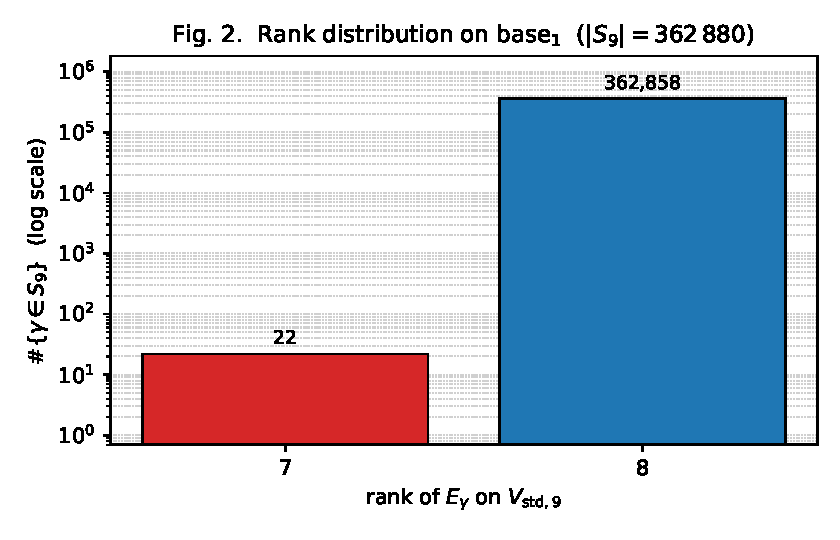
\includegraphics[width=0.7\textwidth]{fig2_rank_distribution.pdf}
   \caption{Rank distribution of $\{\Ehat\}_{\gamma \in S_9}$ on
   \texttt{base1}. Logarithmic vertical axis. The two non-empty bins
   have populations $362{,}858$ (rank $8$) and $22$ (rank $7$);
   no $\gamma \in S_9$ produces $\rank \Ehat \le 6$.}
   \label{fig:rank-distribution}
\end{figure}

\subsection{Four-way exact certification}\label{sec:base1-cert}

Each of the $22$ odd-rank relabelings has been independently certified
by four exact-arithmetic procedures:
\begin{enumerate}[label=(\roman*),leftmargin=*]
   \item \textbf{Integer rank} via Bareiss elimination on $\Egamma \in
   \Z^{9 \times 9}$ followed by truncation to $\Ehat \in
   \Z^{8 \times 8}$;
   \item \textbf{Rational kernel} via SymPy nullspace of $\Ehat$,
   yielding a one-dimensional kernel $\Q$-vector for every
   $\gamma$ in the list, with all entries in $\Z$ after a uniform
   denominator clear-out;
   \item \textbf{Integer Smith normal form} of $\Egamma \in
   \Z^{9 \times 9}$. The elementary-divisor diagonal is rank-$7$ on
   every $\gamma$ in the list (seven nonzero invariants and two
   trailing zeros), but the seventh invariant is \emph{not} uniformly
   $1$: across the $22$ relabelings five distinct diagonals occur,
   namely
   \begin{equation}\label{eq:snf-distribution-base1}
      \begin{array}{ll}
         (1,1,1,1,1,1,1,0,0)  & \text{ on } 10\text{ perms}, \\
         (1,1,1,1,1,1,2,0,0)  & \text{ on }  4\text{ perms}, \\
         (1,1,1,1,1,1,4,0,0)  & \text{ on }  4\text{ perms}, \\
         (1,1,1,1,1,1,3,0,0)  & \text{ on }  2\text{ perms}, \\
         (1,1,1,1,1,2,10,0,0) & \text{ on }  2\text{ perms}.
      \end{array}
   \end{equation}
   In particular only $10/22$ relabelings have torsion-free cokernel
   on $\Z^9 / \mathrm{im}(\Egamma)$; the remaining $12$ carry
   $\Z$-torsion of order $\in \{2, 3, 4, 10\}$. The closed-form
   description of this distribution as a function of $\gamma$ is
   recorded as open problem~(O1) in \S\ref{sec:disc-open};
   \item \textbf{$\mathbb{F}_2$-Smith normal form} of the reduction of
   $\Egamma$ modulo $2$. The integer rank $7$ does \emph{not} lift
   uniformly to $\mathbb{F}_2$: the rank distribution over the $22$
   relabelings is $\{\rank_{\mathbb{F}_2}\!=\!7 : 12,\ 6 : 8,\ 5 :
   2\}$. Twelve relabelings agree mod $2$ (rank $7$); ten drop in
   rank, consistent with the $\Z$-torsion at $2$ in part~(iii).
\end{enumerate}
The four routes are independent in the sense that no two of them
share a common code path past the construction of $\Egamma$. Their
agreement on the $22$-element list (rank $7$ over $\Z$, kernel
$1$-dimensional in $V_{\mathrm{std}}$, integer SNF in the five-class
spectrum~\eqref{eq:snf-distribution-base1}, and the $\mathbb{F}_2$
rank histogram above) rules out single-bug, single-route, and
single-prime artefacts. The per-perm certificates are stored in
\href{../certified/four_way_base1_22.json}{\texttt{four\_way\_base1\_22.json}}
and summarized in Appendix~\ref{app:22-perms}.

\subsection{Scope caveat}\label{sec:base1-scope}

Theorem~\ref{thm:base1-22} concerns \emph{one} Sudoku base under
\emph{all} symbol relabelings. It is \emph{not} a distributional
statement over $\mathrm{Sud}(9)$. Comparable corpus-level statements
require either an exhaustive enumeration of $\mathrm{Sud}(9)$ (out of
reach: $|\mathrm{Sud}(9)| \approx 6.67 \times 10^{21}$ in the sense
of \cite{FelgenhauerJarvis06}) or a sampling caveat
(cf.\ \S\ref{sec:methods}). In particular, the count $22 / 362{,}880
\approx 6.06 \times 10^{-5}$ is the odd-rank rate for \texttt{base1},
not for the population of Sudoku grids.

% =====================================================================
\section{Lower-order calibration}\label{sec:n6n7}
% =====================================================================

The exhaustive analysis of \texttt{base1} at $n = 9$ is one data point
in $\mathrm{Sud}(9)$. To calibrate it against smaller orders, this
section records two facts at $n \in \{6, 7\}$ that together motivate
the structural treatment of \S\S\ref{sec:certificates}--\ref{sec:M19}:
(i) the box constraint does not suppress the $\mathbb{F}_2$-rank
parity proxy at $n = 6$ (i.e.~the rate of grids with
$\rank_{\mathbb{F}_2} \Ehat = n - 1$ is comparable on Sudoku and on
generic Latin squares of order $6$), and (ii) at $n = 7$ the
symmetry group of the simplest odd-rank certificate is dihedral of
order $12$ and embeds inside the box automorphism group $B_3 < S_7$.

\subsection{\texorpdfstring{Roku-Doku at $n = 6$: $\mathbb{F}_2$-rank census}{Roku-Doku at n=6: F2-rank census}}\label{sec:n6}

For $n = 6$, with first row fixed to $(1,2,3,4,5,6)$, the number of
order-$6$ Latin squares is $|\mathrm{LS}(6)|_{\text{first row fixed}}
= 1{,}128{,}960$ and the number of $2 \times 3$ Roku-Doku grids
is $|\mathrm{Sud}(6)|_{\text{first row fixed}} = 39{,}168$.
For each square $L$ in either family, we compute $\rank \Ehat$ at
$\gamma = \mathrm{id}$ over $\mathbb{F}_2$ (the rank-parity proxy of
\cite{HAN-RankParity}) and record the proportion of full-rank-over-$\mathbb{F}_2$
witnesses (\,$\rank_{\mathbb{F}_2} \Ehat = n - 1 = 5$\,).

\begin{proposition}[Roku-Doku exhaustive census]\label{prop:n6-census}
With the first row fixed to $(1,2,3,4,5,6)$,
\begin{align*}
   \#\bigl\{ L \in \mathrm{Sud}(6) : \rank_{\mathbb{F}_2} \Ehat = 5 \bigr\}
      &= 2{,}592 \;\;\;\,\,(=\!6.6177\%), \\
   \#\bigl\{ L \in \mathrm{LS}(6) : \rank_{\mathbb{F}_2} \Ehat = 5 \bigr\}
      &= 69{,}120 \;\;\,(=\!6.1224\%).
\end{align*}
Under the null hypothesis $H_0\!:\;p_{\mathrm{Sud}} = p_{\mathrm{LS}}$ that
the two full-rank-over-$\mathbb{F}_2$ proportions are equal, the standard
pooled two-proportion $z$-test (two-sided, with pooled variance estimator
$\hat p (1-\hat p)\bigl(\tfrac{1}{N_{\mathrm{Sud}}} +
\tfrac{1}{N_{\mathrm{LS}}}\bigr)$ where $\hat p$ is the pooled sample
proportion) yields $z = 4.013706$, with two-sided $p$-value
\begin{equation*}
   p_{\text{two-sided}} \;=\; \mathrm{erfc}\!\bigl(|z|/\sqrt{2}\bigr)
   \;=\; 5.977282 \times 10^{-5}.
\end{equation*}
\end{proposition}

We phrase the conclusion conservatively. The box constraint does
\emph{not} suppress the full-rank-over-$\mathbb{F}_2$ phenomenon at
$n = 6$; in the exhaustive Roku-Doku census, the proportion of
full-rank-over-$\mathbb{F}_2$ witnesses is slightly but significantly
larger than in the Latin-square census.
The full rank distribution at $n = 6$ across the five strata
$\{1, 2, 3, 4, 5\}$ is reported in
\texttt{n6\_odd\_rank\_census.json}.

\subsection{\texorpdfstring{The $n = 7$ group $H_{V_1} \cong D_6$}{The n=7 group HV1 is D6}}\label{sec:n7}

For $n = 7$, fix the laboratory Latin square $L_{V_1}$ of order $7$
recorded in \texttt{scripts/phase\_9\_15.py}, and let $B_3 = S_3 \wr
S_3 \subset S_7$ be the box-permutation group acting on coordinates
(it preserves the partition $\{1,2,3\} \cup \{4,5,6\} \cup \{7\}$ of
the symbol set). Define
\begin{equation}\label{eq:HV1-def}
   H_{V_1} \;:=\; \bigl\{\gamma \in B_3 \;:\;
      \rank \widehat{E}_{\gamma, L_{V_1}} \;=\; 5 \bigr\},
\end{equation}
the intersection of the odd-rank symbol-relabeling locus of
$L_{V_1}$ with $B_3$. Equivalently, $H_{V_1}$ is the
\emph{rank-locus subset} of $B_3$ for the base $L_{V_1}$.

\begin{remark}[$H_{V_1}$ is not a coordinate stabilizer]
\label{rem:HV1-not-coord-stab}
Any vector $v \in \R^7$ with all-distinct coordinates (such as a
linear template $(-3,-2,-1,0,1,2,3) \in A_6$) has trivial coordinate
stabilizer in $S_7$. Hence $H_{V_1}$ cannot be defined as the
coordinate stabilizer of any such vector; it is intrinsically a
\emph{rank-locus} object, defined by the operator condition
\eqref{eq:HV1-def} on $\widehat{E}_{\gamma, L_{V_1}}$.
\end{remark}

\begin{theorem}[Stabilizer at $n = 7$]\label{thm:n7-D6}
The set $H_{V_1}$ defined by~\eqref{eq:HV1-def} satisfies
$|H_{V_1}| = 12$, is closed under composition (hence a subgroup of
$B_3$), and is isomorphic to the dihedral group $D_6 \cong S_3
\times \Z/2$. Explicit generators are
\begin{equation*}
   r \;=\; (3,1,6,4,2,7,5) \in B_3,
   \qquad
   s \;=\; (6,7,3,4,5,1,2) \in B_3,
\end{equation*}
satisfying $r^6 = s^2 = (rs)^2 = e$ and generating $H_{V_1}$ in full.
The rank distribution of $\widehat{E}_{\gamma, L_{V_1}}$ on $B_3$ is
$\{\rank 5 : 12,\ \rank 6 : 36\}$; the rank-$5$ rate inside $B_3$
is $12/48 = 1/4$, against a baseline rate $30/5040 = 1/168$ in
$S_7$, an enrichment ratio of $42$.
\end{theorem}

\begin{proof}[Outline]
The exhaustive enumeration of $\rank \widehat{E}_{\gamma, L_{V_1}}$
for $\gamma \in B_3$ is recorded in
\texttt{n7\_HV1\_D6.json} under \texttt{rank\_distribution\_in\_B3};
this directly gives $|H_{V_1}| = 12$. Closure under composition is
checked element-by-element on the $12$-element list. The element-order
multiset of $H_{V_1}$ is $\{1\!:\!1,\ 2\!:\!7,\ 3\!:\!2,\
6\!:\!2\}$, which uniquely identifies $D_6$ among groups of order
$12$: the alternatives $\Z/12$, $\Z/6 \times \Z/2$, $A_4$, and
$\mathrm{Dic}_3$ all have different order multisets (see
\texttt{n7\_HV1\_D6.json}, field
\texttt{alternatives\_excluded\_by\_order\_distribution}).
Constructively, $r$ has order $6$, $s$ has order $2$, and $s r s =
r^{-1}$ holds in $S_7$ by direct computation; hence $\langle r, s
\rangle = D_6$. The order-$12$ subgroup $\langle r, s \rangle$
coincides with $H_{V_1}$ on enumeration. Membership $r, s \in B_3$
is verified by checking that each preserves the $\{1,2,3\} \cup
\{4,5,6\} \cup \{7\}$ partition; this is implemented in
\href{../scripts/legacy/check_b3_subgroup.py}{\texttt{check\_b3\_subgroup.py}}.
\end{proof}

The Cayley diagram of $\langle r, s \rangle$ is shown in
Figure~\ref{fig:D6-cayley}; it is hexagonal-prismatic, with the
red $6$-cycle $r$ generating the rotational subgroup and the blue
involution $s$ generating the reflection.

\begin{figure}[t]
   \centering
   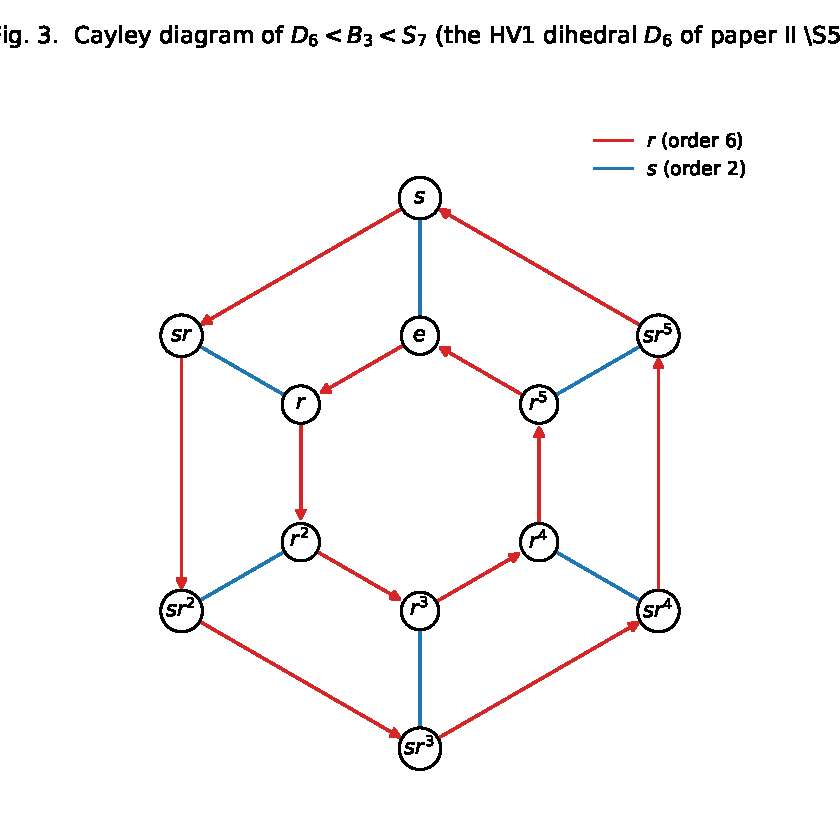
\includegraphics[width=0.55\textwidth]{fig3_D6_cayley.pdf}
   \caption{Cayley diagram of the rank-locus subgroup $H_{V_1} \cong D_6$ at
   $n = 7$. Red edges: generator $r$ of order $6$; blue edges:
   reflection $s$ of order $2$.}
   \label{fig:D6-cayley}
\end{figure}

\subsection{Bridge to rank-parity falsification}\label{sec:parity-bridge}

Theorem~\ref{thm:base1-22} and Proposition~\ref{prop:n6-census}
together show that the parity statement
``$\rank \Ehat \equiv n - 1 \pmod 2$ for every Sudoku grid $L$ and
every $\gamma$'' fails: \texttt{base1} admits $22$ relabelings with
even-corank (odd-rank) $\Ehat$, and $n = 6$ Roku-Doku already
contains over-$\mathbb{F}_2$ rank-$\le 4$ witnesses. These finite
counterexamples are certified inside the present repository and are
the only rank-parity input used below. The broader rank-parity
falsification program is recorded in the sibling working draft
\cite{HAN-RankParity}; here we proceed from the certified
counterexamples to their algebraic structure
(\S\S\ref{sec:certificates}--\ref{sec:autLM19}).

% =====================================================================
\section{\texorpdfstring{Certificates in $\Vstdn$}{Certificates in the standard subspace}}\label{sec:certificates}
% =====================================================================

For every odd-rank pair $(L, \gamma)$, choose a nonzero
$w \in \ker \Ehat$. Lifting $w \in \Q^{n-1}$ along $P_n$ gives a
vector $w \in \Vstdn \cap \Q^n$, and after clearing denominators a
vector in $A_{n-1} = \Vstdn \cap \Z^n$. We refer to such an integer
representative as a \emph{kernel certificate} of $(L, \gamma)$. The
purpose of this section is twofold: first, the Lift Lemma
(Theorem~\ref{thm:lift}) states that the kernel certificate is the
same whether read off $\Egamma$ or off $\gamma(L)$; second, the
support and height taxonomy
(\S\ref{sec:cert-taxonomy}) classifies the kernel certificates that
arise in practice.

\subsection{The Lift Lemma}\label{sec:cert-lift}

\begin{theorem}[Lift Lemma]\label{thm:lift}
Let $L \in \mathrm{LS}(n)$, $\gamma \in S_n$, and $w \in \Vstdn$.
Then
\begin{equation}\label{eq:lift-lemma}
   \Egamma\, w \;=\; 0
   \;\;\iff\;\;
   \gamma(L)\, w \;=\; 0,
\end{equation}
and dually for left kernels: $w^{\!\top} \Egamma = 0 \iff w^{\!\top}
\gamma(L) = 0$.
\end{theorem}

\begin{proof}
For any $w \in \Vstdn$ we have $\one^{\!\top} w = 0$, hence
$J_n w = \one (\one^{\!\top} w) = 0$. Therefore
\begin{equation*}
   \Egamma w \;=\; \gamma(L)\, w \;-\; \frac{n+1}{2} J_n w
              \;=\; \gamma(L)\, w,
\end{equation*}
so the two expressions $\Egamma w$ and $\gamma(L) w$ are identically
equal on $\Vstdn$. The biconditional is immediate, and the dual
statement follows from $w^{\!\top} J_n = 0$.
\end{proof}

\begin{corollary}[Kernel certificates lift to $A_{n-1}$]
\label{cor:cert-in-A}
For every odd-rank pair $(L, \gamma)$, the right kernel of $\Ehat$ is
one-dimensional and lifts to a one-dimensional subspace of $\Vstdn$.
A primitive integer generator of that lift lies in $A_{n-1}$.
\end{corollary}

The integrality of the primitive generator is automatic: the kernel
is a $\Q$-line $\Q v \subseteq \Vstdn$; clearing denominators in $v$
and dividing by the gcd of its entries yields a primitive integer
vector $w \in \Z^n \cap \Vstdn = A_{n-1}$ (with $\gcd_i w_i = 1$),
unique up to sign.

The corollary is verified independently on the $22$ \texttt{base1}
relabelings of \S\ref{sec:base1} and on the $100$ relabelings of
$M_{19}$ scanned in \S\ref{sec:M19}; the relevant histograms are
\begin{equation*}
   \dim_\Q \ker \Egamma|_{\Q^9} = 2 \text{ (}22\text{ times for base$_1$, }100\text{ times for }M_{19}\text{)},
\end{equation*}
\begin{equation*}
   \dim_\Q \ker \Ehat|_{\Vstdn} = 1 \text{ (every odd-rank case)},
\end{equation*}
recorded in \texttt{lift\_lemma\_evidence.json}. The doubled
ambient kernel dimension reflects the fact that $\Q\one \subset
\ker \Egamma$ unconditionally; the lift to $\Vstdn$ removes that
trivial line.

\subsection{Support and height taxonomy}\label{sec:cert-taxonomy}

A kernel certificate $w \in A_{n-1}$ is classified by two coarse
invariants:
\begin{itemize}[leftmargin=*]
   \item the \emph{support} $\mathrm{supp}(w) = \{i : w_i \neq 0\}$,
   in particular the support size $|\mathrm{supp}(w)|$;
   \item the \emph{height} $\|w\|_\infty = \max_i |w_i|$.
\end{itemize}
We say $w$ is \emph{sparse} if $|\mathrm{supp}(w)| \le n/2$ (rounded
up) and \emph{full} otherwise; \emph{low} if $\|w\|_\infty \le n/4$
(rounded down) and \emph{high} otherwise. The two odd-rank orbits at
$n = 9$ used in \S\ref{sec:orbits} arise from a sparse--low
representative
\begin{equation*}
   M \;:=\; (-1, -1, 0, 0, 0, 0, 0, 1, 1) \;\in\; A_8
\end{equation*}
and a sparse--mid representative
\begin{equation*}
   O_6 \;:=\; (-2, -1, 0, 0, 0, 0, 0, 1, 2) \;\in\; A_8.
\end{equation*}
Both have support size $4$, but $\|M\|_\infty = 1$ versus
$\|O_6\|_\infty = 2$; this height invariant is sufficient to separate
the two $G^*$-orbits of \S\ref{sec:orbits}.

\subsection{Combinatorial identities from kernel vectors}
\label{sec:cert-identities}

Each kernel certificate $w \in A_{n-1}$ encodes a linear identity
$\gamma(L)\, w = 0$, which expands as
\begin{equation}\label{eq:cert-identity}
   \sum_{j=1}^{n} w_j \, \gamma(L_{ij}) \;=\; 0
   \qquad \text{for every row $i$ of $L$,}
\end{equation}
together with the column-wise dual. For sparse certificates the
identity reduces to a relation among at most $|\mathrm{supp}(w)|$
column entries of $\gamma(L)$ per row. The resulting identity is
\emph{Sudoku-specific} only insofar as the certificate $w$ arises;
on a generic Latin square no such $w$ exists.

% =====================================================================
\section{\texorpdfstring{Orbit structure and $A_8$ saturation}{Orbit structure and A8 saturation}}\label{sec:orbits}
% =====================================================================

We now restrict to $n = 9$ and analyze the $G^*$-orbits of the kernel
certificates of \S\ref{sec:cert-taxonomy}. For every $n$ used below,
we take
\begin{equation*}
   G^*_n \;:=\; S_n \times \{\pm 1\},
   \qquad
   (\sigma,\varepsilon)\cdot v
   \;:=\; \varepsilon\,(v_{\sigma^{-1}(1)},\ldots,v_{\sigma^{-1}(n)})
\end{equation*}
on $A_{n-1}\subset \Z^n$. Thus $G^*_n$ is the signed coordinate-
permutation group generated by coordinate permutations and global
sign. When $n=9$ we write $G^*$ for $G^*_9$.

\subsection{Sparse--low and sparse--mid orbits}\label{sec:orbit-classes}

Acting on $A_8$ by signed permutation of coordinates, $G^*$ produces
two finite orbits of the representatives $M$ and $O_6$:
\begin{equation*}
   \mathrm{orb}(M) \subseteq A_8,
   \qquad |\mathrm{orb}(M)| = 756,
\end{equation*}
\begin{equation*}
   \mathrm{orb}(O_6) \subseteq A_8,
   \qquad |\mathrm{orb}(O_6)| = 3024.
\end{equation*}
The two orbits are disjoint (the height invariant
$\|\cdot\|_\infty$ separates them) and each is a finite set of
integer vectors of $\Vstdn$.

\subsection{Lattice generated by an orbit}\label{sec:lattice-orbit}

For an orbit $\mathcal{O} \subseteq A_8$, write
\begin{equation*}
   \Lambda_{\mathcal{O}} \;:=\; \Z\langle \mathcal{O} \rangle
\end{equation*}
for the integer lattice generated by $\mathcal{O}$ inside $\Vstdn$.
By construction $\Lambda_{\mathcal{O}} \subseteq A_8$. The
\emph{saturation} statement is the equality $\Lambda_{\mathcal{O}}
= A_8$; equivalently, the elementary divisors of any matrix whose
columns are vectors of $\mathcal{O}$ spanning $\Lambda_{\mathcal{O}}$
should all equal $1$ (rank $8$).

\begin{theorem}[$A_8$ saturation]\label{thm:A8-saturation}
At $n = 9$,
\begin{equation*}
   \Lambda_{M} \;=\; \Lambda_{O_6} \;=\; A_8 \;=\; \Vstdn \cap \Z^9.
\end{equation*}
Both $\Lambda_M$ and $\Lambda_{O_6}$ have rank $8$ and elementary
divisors $(1, 1, 1, 1, 1, 1, 1, 1)$.
\end{theorem}

\begin{proof}[Outline]
For each orbit $\mathcal{O} \in \{\mathrm{orb}(M),\mathrm{orb}(O_6)\}$,
the entire orbit is used as a (redundant) spanning set: the orbit
vectors are stacked into the rows of an integer matrix of shape
$(|\mathcal{O}|, 9)$, namely $(756, 9)$ for $\mathrm{orb}(M)$ and
$(3024, 9)$ for $\mathrm{orb}(O_6)$. Smith normal form over $\Z$ is
applied via SymPy. In both cases the elementary divisors are
$(1,1,1,1,1,1,1,1)$ (eight $1$'s, recorded in fields
\texttt{outputs.Lambda\_M.elementary\_divisors} and
\texttt{outputs.Lambda\_O6.elementary\_divisors} of
\texttt{A8\_saturation.json}), confirming rank $8$ and full
saturation of $A_8$ inside $\Vstdn$. The implementation is in
\href{../scripts/legacy/phase_9_18_S9q_beta_lattice.py}{\texttt{phase\_9\_18\_S9q\_beta\_lattice.py}};
the certified output is \texttt{A8\_saturation.json}.
\end{proof}

\begin{figure}[t]
   \centering
   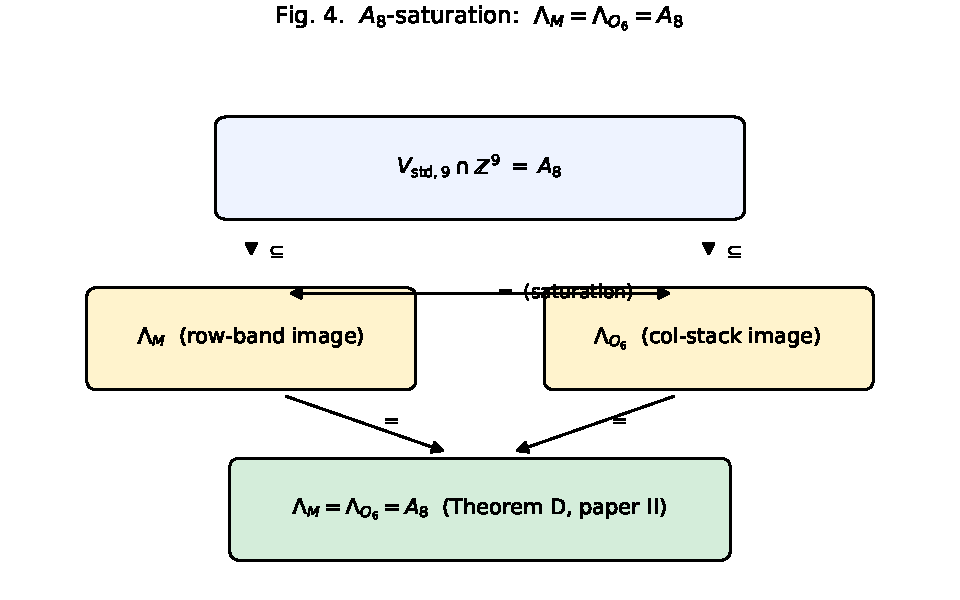
\includegraphics[width=0.7\textwidth]{fig4_A8_saturation.pdf}
   \caption{Schematic of the saturation $\Lambda_M = \Lambda_{O_6} =
   A_8$. Both sparse--low and sparse--mid orbits already saturate the
   ambient root lattice $A_8$ at the level of $\Z$-spans.}
   \label{fig:A8-saturation}
\end{figure}

\subsection{\texorpdfstring{The $\{M, O_6\}$ dichotomy at $n = 9$}{The M/O6 dichotomy at n=9}}\label{sec:dichotomy-n9}

Theorem~\ref{thm:A8-saturation} promotes the height taxonomy of
\S\ref{sec:cert-taxonomy} to a structural statement: at $n = 9$, the
sparse-template odd-rank certificates of $\Egamma$ split into exactly
two $G^*$-orbits, with representatives $M$ (sparse--low,
$|\mathrm{orb}| = 756$) and $O_6$ (sparse--mid, $|\mathrm{orb}| =
3024$), and both orbits saturate $A_8$. The general-$n$ extension of
this dichotomy is the content of \S\ref{sec:dichotomy}.

% =====================================================================
\section{\texorpdfstring{The $M_{19}$ laboratory and Hessian symmetry}{The M19 laboratory and Hessian symmetry}}\label{sec:M19}
% =====================================================================

The Sudoku grid $M_{19}$ is the laboratory base under which the
bilateral symmetry of $\Egamma$ is most cleanly visible at $n = 9$.
The grid itself is
\begin{equation}\label{eq:M19-grid}
   M_{19} \;=\;
   \begin{pmatrix}
      2 & 6 & 3 & 8 & 1 & 5 & 4 & 7 & 9 \\
      4 & 9 & 8 & 3 & 6 & 7 & 2 & 5 & 1 \\
      7 & 5 & 1 & 4 & 9 & 2 & 3 & 6 & 8 \\
      8 & 2 & 5 & 1 & 3 & 9 & 6 & 4 & 7 \\
      6 & 4 & 7 & 5 & 2 & 8 & 1 & 9 & 3 \\
      3 & 1 & 9 & 6 & 7 & 4 & 5 & 8 & 2 \\
      5 & 7 & 4 & 2 & 8 & 1 & 9 & 3 & 6 \\
      9 & 3 & 2 & 7 & 5 & 6 & 8 & 1 & 4 \\
      1 & 8 & 6 & 9 & 4 & 3 & 7 & 2 & 5
   \end{pmatrix}.
\end{equation}
This grid is recorded byte-equal in the input field of
\path{M19_audit.json} and \path{M19_KL_KR_3sq_Q8.json}; it
emerged from a uniform random search over Sudoku bases, conducted
as described in \S\ref{sec:methods}, as the candidate with the
largest observed odd-rank relabeling count among the sampled grids.
We make no claim that $M_{19}$ is globally maximal in this respect,
nor that it is unique up to isomorphism among grids with $100$
odd-rank relabelings; it is fixed here as the laboratory base on
which the bilateral Hessian symmetry of \S\ref{sec:M19-hessian} is
most cleanly observed.

\subsection{\texorpdfstring{Exhaustive $S_9$ audit of $M_{19}$}{Exhaustive S9 audit of M19}}\label{sec:M19-audit}

We separate three distinct objects that all live on the laboratory base
$M_{19}$ and that an earlier draft of this paper conflated into a single
symbol $\Gamma^*_{M_{19}}$.

\begin{definition}[Three sets on $M_{19}$]\label{def:M19-three-sets}
At the laboratory base $M_{19}$ we define:
\begin{enumerate}
   \item[\rm (a)] The exhaustive \emph{rank locus}
   \begin{equation*}
      \GrankM \;:=\; \bigl\{\gamma \in S_9 : \rank \widehat{E}_{\gamma, M_{19}} = 7\bigr\},
   \end{equation*}
   the set of all relabelings that drop the rank of the centered operator
   below the generic value $8$.
   \item[\rm (b)] The \emph{Hessian-class subset}
   \begin{equation*}
      \GMninetn \;:=\; \bigl\{\gamma \in \GrankM :
         \ker \Egamma \cap \Vstdn \;=\; \mathbb{Z}\langle u^*_9 \rangle \bigr\},
   \end{equation*}
   the relabelings whose centered kernel collapses to a fixed shared
   primitive direction $u^*_9$ (defined below).
   \item[\rm (c)] The \emph{ambient coordinate stabilizer}
   \begin{equation*}
      \StabUnine \;\subset\; S_9,
   \end{equation*}
   the coordinate stabilizer of $u^*_9$ under the standard action of
   $S_9$ on $\mathbb{Z}^9$.
\end{enumerate}
The three sets are pairwise distinct as cardinalities and as combinatorial
objects: (a) is a set of permutations, (b) is a proper subset of (a), and
(c) is a subgroup of $S_9$.
\end{definition}

Throughout the sequel, $\GMninetn$ always denotes the Hessian-class
subset in Definition~\ref{def:M19-three-sets}(b), not the full
rank-locus $\GrankM$ in Definition~\ref{def:M19-three-sets}(a). Thus
$|\GMninetn| = 72$ and $|\GrankM| = 100$ are intentionally distinct
certified quantities.

\begin{proposition}[Audit of $M_{19}$]\label{prop:M19-audit}
The exhaustive $S_9$-audit of $M_{19}$ yields:
\begin{enumerate}
   \item[\rm (i)] $|\GrankM| = 100$ out of $|S_9| = 9! = 362{,}880$ (rank
   distribution $\{8 : 362{,}780,\ 7 : 100\}$);
   \item[\rm (ii)] the Hessian-class subset has size $|\GMninetn| = 72$,
   with shared primitive kernel direction
   \begin{equation*}
      u^*_9 \;=\; (-2,\, -2,\, -2,\, 1,\, 1,\, 1,\, 1,\, 1,\, 1) \;\in\; A_8;
   \end{equation*}
   the $|\GrankM \setminus \GMninetn| = 28$ residual relabelings split
   into $14$ smaller kernel orbits (full orbit count $|\GrankM|$ in
   $S_9$ via canonicalization of the kernel template: $15$);
   \item[\rm (iii)] the ambient coordinate stabilizer satisfies
   \begin{equation*}
      \StabUnine \;\cong\; S_3 \times S_6,
      \qquad |\StabUnine| \;=\; 3!\cdot 6! \;=\; 4320,
   \end{equation*}
   since $u^*_9$ has value-multiplicities $\{-2 : 3,\ 1 : 6\}$.
\end{enumerate}
\end{proposition}

\begin{proof}[Outline]
The rank distribution $\{8: 362{,}780,\ 7: 100\}$ is recomputed by an
exhaustive two-stage scan: (a) NumPy float rank flag every $\gamma$ with
$\rank \widehat{E}_{\gamma, M_{19}} < 8$ ($100$ candidates in
${\sim}15$ s); (b) Sympy exact integer rank verification on every
candidate, returning rank $7$ for all $100$. The full list of $100$
permutations is shipped in
\texttt{M19\_100\_perms\_recovered.json} (sha256 in
\texttt{MANIFEST.sha256}); the script is
\texttt{recover\_M19\_100\_perms.py}. Statement (ii) is read from
\texttt{phase\_9\_18\_S9x\_results.json} via the canonicalization of the
kernel template, and the $72$-element Hessian class is checked subset of
the $100$ rank-$7$ list directly. Statement (iii) is the orbit-stabilizer
calculation: $u^*_9$ has the multiset $\{-2,-2,-2,1,1,1,1,1,1\}$ with
multiplicities $\{-2 : 3,\ 1 : 6\}$, hence its $S_9$-coordinate
stabilizer is $S_3 \times S_6$ of order $4320$. The orbit of $u^*_9$ in
$S_9 \cdot u^*_9$ has size $9!/4320 = 84$, of which only one element is
realized as a kernel direction over the $\GMninetn$ certificates.
\end{proof}

\begin{remark}[The number $4320$ is an ambient stabilizer, not an orbit]
\label{rem:4320-not-orbit}
The number $4320$ is the order of the ambient coordinate stabilizer
$\StabUnine = \mathrm{Stab}_{S_9}(u^*_9) \cong S_3 \times S_6$, an
algebraic invariant of the kernel direction $u^*_9$. It is \emph{not}
the cardinality of any of $\GrankM$, $\GMninetn$, or any orbit of
$\KL \times \KR$ on a rank-locus set; indeed
$|\KL \times \KR| = 72\cdot 72 = 5184$ is not divisible by $4320$
(ratio $6/5$). The three numbers $|\GrankM| = 100$, $|\GMninetn| = 72$,
$|\StabUnine| = 4320$ live in distinct categories (rank-locus size,
Hessian-class size, ambient stabilizer order) and should not be
identified.
\end{remark}

\subsection{\texorpdfstring{Single-coset structure of the Hessian class $\GMninetn$}{Single-coset structure of the Hessian class}}
\label{sec:M19-coset}

We now identify the symmetries of the Hessian-class subset $\GMninetn$.
Define
\begin{align}
   \KL &\;:=\; \bigl\{\pi \in S_9 \;:\; \pi \cdot \GMninetn \;\subseteq\;
      \GMninetn\bigr\}, \label{eq:KL-def}\\
   \KR &\;:=\; \bigl\{\pi \in S_9 \;:\; \GMninetn \cdot \pi \;\subseteq\;
      \GMninetn\bigr\}. \label{eq:KR-def}
\end{align}
By a direct exhaustive computation in $S_9$ (recorded under fields
\texttt{K\_L\_size}, \texttt{K\_R\_size},
\texttt{left\_coset\_test\_PASS}, \texttt{right\_coset\_test\_PASS} of
\texttt{M19\_audit.json}), both $\KL$ and $\KR$ are subgroups of $S_9$
of order $72$, and $\GMninetn$ is simultaneously a single left coset of
$\KL$ and a single right coset of $\KR$.

\begin{theorem}[Single-coset structure of $\GMninetn$]
\label{thm:M19-coset}
The Hessian-class subset $\GMninetn$ has cardinality $72$, and there
exists $\gamma_0 \in \GMninetn$ such that
\begin{equation}\label{eq:single-coset}
   \GMninetn \;=\; \KL \cdot \gamma_0 \;=\; \gamma_0 \cdot \KR,
\end{equation}
with $|\KL| = |\KR| = 72$. The two subgroups intersect trivially,
$\KL \cap \KR = \{e\}$, but they are conjugate in $S_9$ via $\gamma_0$:
\begin{equation}\label{eq:KL-conj-KR}
   \KL \;=\; \gamma_0\, \KR\, \gamma_0^{-1}.
\end{equation}
Equivalently, the double coset $\KL \cdot \gamma_0 \cdot \KR$ has
cardinality $72$, which by the standard double-coset formula
\begin{equation*}
   |\KL\, \gamma_0\, \KR| \;=\;
   \frac{|\KL|\cdot|\KR|}{|\KL \cap \gamma_0\, \KR\, \gamma_0^{-1}|}
\end{equation*}
forces $|\KL \cap \gamma_0\, \KR\, \gamma_0^{-1}| = 72 = |\KL| = |\KR|$,
i.e.\ \eqref{eq:KL-conj-KR}.
\end{theorem}

\begin{proof}[Outline]
The orders $|\KL| = |\KR| = 72$ and the equality
$\GMninetn = \KL \cdot \gamma_0 = \gamma_0 \cdot \KR$ are read off the
exhaustive set-stabilizer computation recorded in
\texttt{M19\_audit.json} (fields \texttt{left\_coset\_test\_PASS},
\texttt{right\_coset\_test\_PASS}, \texttt{K\_L\_size},
\texttt{K\_R\_size}). The intersection $\KL \cap \KR$ is computed as a
finite set in $S_9$ and returns the singleton $\{e\}$; this is recorded
in \texttt{M19\_KL\_KR\_3sq\_Q8.json} under
\texttt{K\_L\_inter\_K\_R\_size}. The conjugacy
$\KL = \gamma_0 \KR \gamma_0^{-1}$ is then forced by the double-coset
size identity: with $|\KL\,\gamma_0\,\KR| = |\GMninetn| = 72$ and
$|\KL| = |\KR| = 72$, one gets
$|\KL \cap \gamma_0 \KR \gamma_0^{-1}| = 72$, hence
$\KL = \gamma_0 \KR \gamma_0^{-1}$. The corresponding boolean
\texttt{Y2\_conjugate\_via\_pi0} is recorded \texttt{true} in
\texttt{M19\_KL\_KR\_3sq\_Q8.json}.
\end{proof}

A schematic of the single-coset structure is shown in
Figure~\ref{fig:M19-coset}.

\begin{figure}[t]
   \centering
   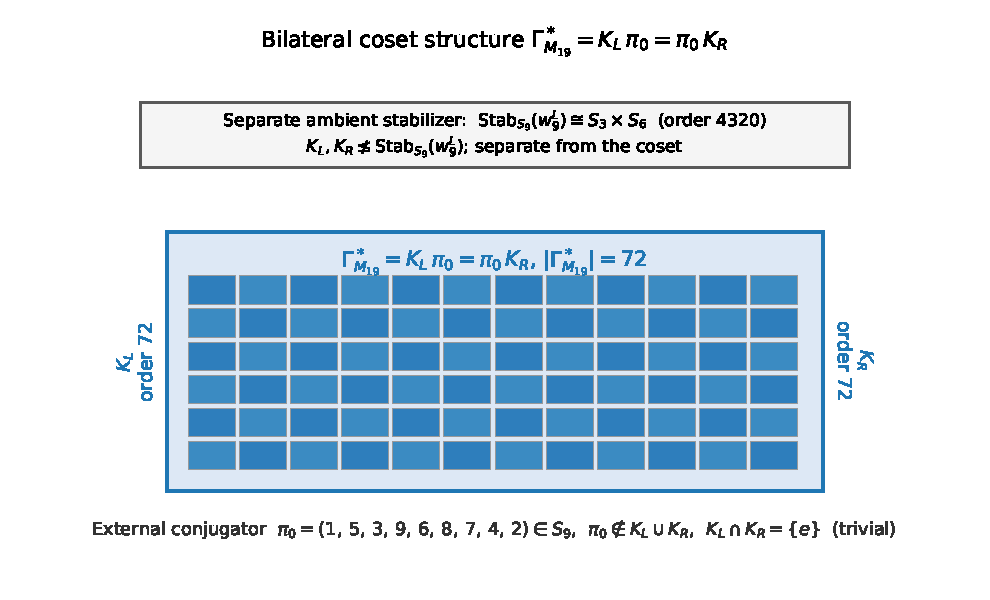
\includegraphics[width=0.7\textwidth]{fig5_M19_coset_structure.pdf}
   \caption{Schematic of the single-coset structure of $\GMninetn$. The
   left axis is the $|\KL| = 72$ direction; $\GMninetn = \KL \cdot
   \gamma_0$ is itself a single left $\KL$-coset of cardinality $72$.
   The structural permutation $\gamma_0 \in \GMninetn$ also satisfies
   $\GMninetn = \gamma_0 \cdot \KR$; the conjugation
   $\KL = \gamma_0\, \KR\, \gamma_0^{-1}$ identifies the two Hessian
   sides.}
   \label{fig:M19-coset}
\end{figure}

\subsection{\texorpdfstring{Hessian identification: $\KL \cong \KR \cong 3^2{:}Q_8$}{Hessian identification: KL and KR are 3 squared colon Q8}}
\label{sec:M19-hessian}

\begin{theorem}[Hessian symmetry of $M_{19}$]\label{thm:M19-hessian}
At $L = M_{19}$ and $n = 9$, the left and right Hessian symmetry
groups satisfy
\begin{equation*}
   \KL \;\cong\; \KR \;\cong\; \HesGroup
   \;=\; \mathrm{SmallGroup}(72, 41).
\end{equation*}
Both have order $72$, exponent $6$, derived series of orders
$(72, 18, 9, 1)$, abelianization $\Z/4$, trivial centre, and
$9$ conjugacy classes. The element-order distribution is
$\{1\!:\!1,\ 2\!:\!21,\ 3\!:\!8,\ 4\!:\!18,\ 6\!:\!24\}$.
$\KL$ and $\KR$ are not equal as subgroups of $S_9$ (their
intersection is trivial: $\KL \cap \KR = \{e\}$), but they are
conjugate inside $S_9$ via an external structural permutation
$\pi_0 \in S_9 \setminus (\KL \cup \KR)$ characterized in
Remark~\ref{rem:pi0}.
\end{theorem}

\begin{proof}[Outline of identification]
The order $|\KL| = 72$ rules out abelian groups and groups of
exponent $\le 2$. The derived series $(72, 18, 9, 1)$ identifies
$\KL$ as solvable of derived length $3$. Among the $50$ groups of
order $72$ classified in
\cite{ConwaySloaneSPLAG, GAPSmallGroups, ATLASsmallorder}, the
combination of exponent $6$, abelianization $\Z/4$, trivial centre,
$9$ conjugacy classes, and the element-order multiset
$\{1\!:\!1,\ 2\!:\!21,\ 3\!:\!8,\ 4\!:\!18,\ 6\!:\!24\}$
uniquely picks out $\mathrm{SmallGroup}(72, 41) \cong 3^2 \rtimes Q_8$,
the unique non-abelian extension of $Q_8$ by $(\Z/3)^2$ of Hessian
type \cite[Ch.~10]{ConwaySloaneSPLAG}. Uniqueness of the match was
checked by querying the \texttt{GAP} \texttt{SmallGroups} library
\cite{GAPSmallGroups} over $k \in \{1,\ldots,50\}$ via the standard
predicates \texttt{Exponent}, \texttt{AbelianInvariants(DerivedSubgroup)},
\texttt{Centre}, \texttt{NrConjugacyClasses}, and element-order multiset:
the conjunction of all five invariants is met by exactly one entry,
namely $k = 41$. The full identification certificate, including the
$8$ explicit generator permutations, is recorded in
\texttt{M19\_KL\_KR\_3sq\_Q8.json}.
\end{proof}

\begin{remark}[Structural permutation $\pi_0$]\label{rem:pi0}
The canonical structural permutation conjugating $\KR$ to $\KL$ is
the lex-minimum element of the bilateral coset $\Gamma^{*}_{M_{19}}
= \KL \gamma_0 = \gamma_0 \KR$, namely
\begin{equation}\label{eq:pi0-perm}
   \pi_0 \;=\; (1,\, 5,\, 3,\, 9,\, 6,\, 8,\, 7,\, 4,\, 2)
   \;\in\; S_9
   \qquad\text{(one-line notation).}
\end{equation}
This $\pi_0$ is \emph{not} an element of $\KL$ nor of $\KR$; in
particular it is not one of the eight generators listed in
\texttt{outputs.K\_L\_generators\_perms}. It satisfies
$\pi_0 \KR \pi_0^{-1} = \KL$ and is the witness implementing the
output field \texttt{Y2\_conjugate\_via\_pi0 = true}; the entire
coset $\Gamma^{*}_{M_{19}}$ admits the bilateral factorisation
$\Gamma^{*}_{M_{19}} = \pi_0 \KR = \KL \pi_0$. The certificate file
\texttt{M19\_KL\_KR\_3sq\_Q8.json} records both the eight-generator
presentation of $\KL$ and the explicit value of $\pi_0$ in its
\texttt{outputs.pi0\_perm} field.
\end{remark}

\begin{remark}[Hessian groups in $S_9$]\label{rem:hessian-context}
The group $3^2{:}Q_8$ is the classical \emph{Hessian group} of
order $72$, identified by Hesse in the context of the inflection
configuration of a smooth plane cubic curve. Its appearance here is
not a priori expected: it arises from a purely Sudoku-driven
construction, with no intervening cubic geometry. The Sudoku
specificity of this realization is investigated in
\S\ref{sec:autLM19}.
\end{remark}

% =====================================================================
\section{\texorpdfstring{Stabilizer dichotomy $\{M_n, O_n\}$}{Stabilizer dichotomy Mn/On}}\label{sec:dichotomy}
% =====================================================================

We now lift the $\{M, O_6\}$ structure of \S\ref{sec:dichotomy-n9} to
a one-parameter family of representatives at general $n$. For
$n \ge 5$, define the canonical sparse--low and sparse--mid integer
vectors of $A_{n-1}$ by
\begin{equation*}
   M_n \;:=\; \bigl(-1,\, -1,\, \underbrace{0,\dots,0}_{n-4},\, 1,\, 1\bigr),
   \qquad
   O_n \;:=\; \bigl(-2,\, -1,\, \underbrace{0,\dots,0}_{n-4},\, 1,\, 2\bigr).
\end{equation*}
At $n = 9$, $M_9 = M$ and $O_9 = O_6$ in the notation of
\S\ref{sec:cert-taxonomy}. The next two results identify the $G^*_n$-stabilizers
of $M_n$ and $O_n$ analytically at $n \in \{7, 9, 11\}$ and verify
the orbit-size and stabilizer-order formulas exhaustively for
$5 \le n \le 13$.

\subsection{\texorpdfstring{Exhaustive verification at $5 \le n \le 13$}{Exhaustive verification at 5 <= n <= 13}}
\label{sec:dichotomy-exhaustive}

\begin{proposition}[Exhaustive dichotomy]
\label{prop:dichotomy-exhaustive}
For every integer $n$ with $5 \le n \le 13$,
\begin{equation*}
   |\Stab_{G^*_n}(M_n)| \;=\; 8 \,(n-4)!,
   \qquad
   |\Stab_{G^*_n}(O_n)| \;=\; 2 \,(n-4)!,
\end{equation*}
and
\begin{equation*}
   |\mathrm{orb}_{G^*_n}(M_n)| \;=\; \frac{n(n-1)(n-2)(n-3)}{4},
\end{equation*}
\begin{equation*}
   |\mathrm{orb}_{G^*_n}(O_n)| \;=\; n(n-1)(n-2)(n-3).
\end{equation*}
The orbit-distance $d_{M_n}(\mathrm{orb}(O_n)) = 2$, and
$\Lambda_{M_n} = \Lambda_{O_n} = A_{n-1}$ (saturation, elementary
divisors all $1$).
\end{proposition}

The proposition is verified by direct computation in
\href{../scripts/legacy/phase_9_18_S9q_gamma1.py}{\texttt{phase\_9\_18\_S9q\_gamma1.py}};
total wall-time $\approx 31$ seconds. The certified output is
\texttt{stabilizers\_5\_to\_13.json}.

\subsection{\texorpdfstring{Analytic identification at $n \in \{7, 9, 11\}$}{Analytic identification at n in {7,9,11}}}
\label{sec:dichotomy-analytic}

\begin{theorem}[Analytic dichotomy at $n \in \{7, 9, 11\}$]
\label{thm:dichotomy-analytic}
For each $n \in \{7, 9, 11\}$,
\begin{equation*}
   \Stab_{G^*_n}(M_n) \;\cong\; D_4 \times S_{n-4},
   \qquad
   \Stab_{G^*_n}(O_n) \;\cong\; \Z/2 \times S_{n-4},
\end{equation*}
and the integer hulls satisfy $\Lambda_{M_n} = \Lambda_{O_n} =
A_{n-1}$.
\end{theorem}

\begin{proof}[Outline]
At each $n \in \{7,9,11\}$, the stabilizer of $M_n$ in $G^*_n$
admits a canonical short exact sequence
\begin{equation*}
   1 \;\to\; \ker \psi \;\to\; \Stab_{G^*_n}(M_n)
   \;\xrightarrow{\psi}\; S_{n-4} \;\to\; 1,
\end{equation*}
where $\psi$ is the restriction to the zero-coordinate block of $M_n$
and $\ker \psi$ acts only on the four nonzero coordinates. The
sequence splits because the inclusion $S_{n-4} \hookrightarrow
G^*_n$ on the zero block is a section. Hence
\begin{equation*}
   \Stab_{G^*_n}(M_n) \;\cong\; \ker \psi \,\rtimes_{\mathrm{triv}}\, S_{n-4}
   \;=\; \ker \psi \,\times\, S_{n-4},
\end{equation*}
and the order of $\ker \psi$ is $8 = |\Stab_{G^*_n}(M_n)| /
(n-4)!$ by Proposition~\ref{prop:dichotomy-exhaustive}.

To identify $\ker \psi$ as $D_4$ rather than as one of the four other
groups of order $8$, we compute the order distribution of $\ker \psi$
and obtain
\begin{equation*}
   \{1\!:\!1,\ 2\!:\!5,\ 4\!:\!2\},
\end{equation*}
which uniquely separates $D_4$ from $Q_8$ ($\{1\!:\!1, 2\!:\!1,
4\!:\!6\}$), $\Z/8$ ($\{1\!:\!1, 2\!:\!1, 4\!:\!2, 8\!:\!4\}$),
$\Z/4 \times \Z/2$ ($\{1\!:\!1, 2\!:\!3, 4\!:\!4\}$), and
$(\Z/2)^3$ ($\{1\!:\!1, 2\!:\!7\}$).

The argument for $\Stab_{G^*_n}(O_n) \cong \Z/2 \times S_{n-4}$ is
identical, with $\ker \psi$ of order $2$ and order distribution
$\{1\!:\!1,\ 2\!:\!1\}$ (the unique group of order $2$).

The lattice saturation $\Lambda_{M_n} = \Lambda_{O_n} = A_{n-1}$ is
read from the elementary divisors of the orbit-Gram matrix, all
equal to $1$ at $n \in \{7,9,11\}$.
\end{proof}

The full witness fingerprint, including the order-multiset checks
and the alternative-exclusion list, is in
\texttt{dichotomy\_n7\_n9\_n11.json}.

\subsection{\texorpdfstring{General-$n$ conjecture}{General-n conjecture}}\label{sec:dichotomy-general}

\begin{conjecture}[General-$n$ dichotomy]\label{conj:universal-dichotomy}
For every integer $n \ge 5$,
\begin{equation*}
   \Stab_{G^*_n}(M_n) \;\cong\; D_4 \times S_{n-4},
   \qquad
   \Stab_{G^*_n}(O_n) \;\cong\; \Z/2 \times S_{n-4},
\end{equation*}
and $\Lambda_{M_n} = \Lambda_{O_n} = A_{n-1}$.
\end{conjecture}

The evidence base for Conjecture~\ref{conj:universal-dichotomy} is
the union of Theorem~\ref{thm:dichotomy-analytic} (analytic, $n \in
\{7,9,11\}$) and Proposition~\ref{prop:dichotomy-exhaustive}
(exhaustive computational, $5 \le n \le 13$). No further evidence
is claimed in this paper.

The upper bound $n = 13$ on the exhaustive scan reflects the
computational scope of the present work, not a fundamental obstruction:
the orbit and elementary-divisor checks for $n = 14, 15$ are
tractable in principle but require a one- to two-order-of-magnitude
increase in CPU time and were not run for this paper. We deliberately
stop the exhaustive ledger at $n = 13$ rather than extend the
evidence in a piecemeal way.

% =====================================================================
\section{Sudoku-specificity beyond Latin-square autotopisms}
\label{sec:autLM19}
% =====================================================================

The Hessian group $\KL \cong 3^2{:}Q_8$ identified at $M_{19}$ is
not a familiar Latin-square invariant. The classical group attached
to a Latin square $L$ is its autotopism group $\Aut(L)$,
i.e.\ the set of triples $(\alpha, \beta, \gamma) \in S_n^3$ that
preserve $L$ in the sense $L_{\alpha(i)\,\beta(j)} =
\gamma(L_{ij})$. Even when $L$ is taken as a Sudoku grid, the
operative group from the Latin-square literature is $\Aut(L)$ or one
of its standard refinements (paratopism, principal isotopy, see
\cite{Wanless11, SVW12, AutotopismsPartialLatin20}). This section
shows that for $L = L_{M_{19}}$ the autotopism group is trivial,
hence cannot be the source of $\KL$.

\subsection{\texorpdfstring{Triviality of $\Aut(L_{M_{19}})$}{Triviality of Aut(LM19)}}\label{sec:aut-triv}

Let $L_{M_{19}}$ denote the Latin square underlying $M_{19}$; that
is, the $9 \times 9$ array of \eqref{eq:M19-grid} viewed without
its Sudoku/box structure.

\begin{theorem}[$\Aut(L_{M_{19}})$ is trivial]\label{thm:aut-LM19-trivial}
The autotopism group of $L_{M_{19}}$ has order $1$:
\begin{equation*}
   |\Aut(L_{M_{19}})| \;=\; 1.
\end{equation*}
\end{theorem}

\begin{proof}[Outline]
The full $9!^3 = 4.79 \times 10^{16}$ triple-search is reduced
algorithmically: fix $\gamma \in S_9$, and for each fixed
$\gamma$ search the $9!^2$ pairs $(\alpha, \beta)$ such that
$L_{\alpha(i),\beta(j)} = \gamma(L_{ij})$ via a constrained
backtracking that prunes on the first row. The exhaustive scan over
all $9! = 362{,}880$ values of $\gamma$ yields the trivial autotopism
$(\mathrm{id}, \mathrm{id}, \mathrm{id})$ and no other; the total
wall-clock runtime is $68.79$~s on a single thread (Python~3.14,
Windows~x64), recorded in field \texttt{outputs.elapsed\_s} of
\texttt{Aut\_LM19\_trivial.json}, and the run is byte-deterministic
under the fixed seed declared in \texttt{seed} of the same file.
\end{proof}

\begin{corollary}[$\KL$ is not an autotopism group]
\label{cor:KL-not-autotopism}
The Hessian symmetry group $\KL$ of $M_{19}$ is not the image of any
autotopism subgroup of $L_{M_{19}}$. In particular, $|\KL| = 72 \neq
1 = |\Aut(L_{M_{19}})|$.
\end{corollary}

\begin{proof}
Any homomorphic image of $\Aut(L_{M_{19}})$ in $S_9$ has order
$\le |\Aut(L_{M_{19}})| = 1$ by Theorem~\ref{thm:aut-LM19-trivial}.
But $|\KL| = 72$ by Theorem~\ref{thm:M19-hessian}, so $\KL$ cannot
be such an image.
\end{proof}

\subsection{\texorpdfstring{Box / $A_8$ origin of $\KL$}{Box / A8 origin of KL}}\label{sec:KL-origin}

Since $\KL$ is not generated by autotopisms of $L_{M_{19}}$, its
$72$ elements must arise from a Sudoku-grid feature beyond the
Latin-square structure. The Box Band Lemma
(Theorem~\ref{thm:box-band}) and the $A_8$ saturation
(Theorem~\ref{thm:A8-saturation}) together provide the natural
candidate: the box partition contributes $9$ extra linear
constraints \eqref{eq:bbl-formal} on $\Egamma$, and the kernel
certificates lie in $A_8$, on which the Hessian group of order $72$
acts by classical projective construction
\cite[Ch.~10]{ConwaySloaneSPLAG}.

We do not claim a structural derivation $\KL = $ ``Sudoku
$\Rightarrow$ $A_8 \Rightarrow$ Hessian'' in this paper.
Theorem~\ref{thm:aut-LM19-trivial} merely closes the obvious
alternative: the symmetry is genuinely Sudoku-specific in the sense
that no Latin-square autotopism produces it. A structural derivation
is recorded as Open Problem in \S\ref{sec:disc-open}.

% =====================================================================
\section{Computational methods and reproducibility}\label{sec:methods}
% =====================================================================

The four main theorems and the supporting propositions of this paper
are obtained from a combination of analytic argument and exhaustive
exact-arithmetic computation. This section records the methodology
and points to the certified reproducibility package.

\smallskip
\noindent\textbf{Exact arithmetic.} All ranks, kernels, Smith normal
forms, and group-order computations are performed in exact
arithmetic over $\Z$ or $\Q$, never in floating point. The integer
rank computations use Bareiss fraction-free elimination
\cite{Bareiss68}; rational nullspaces use SymPy RREF; Smith normal
forms use the standard $\Z$-elementary-divisor algorithm. Each
odd-rank report is independently cross-checked at primes $p \in
\{2, 3, 5, 7\}$, the agreement of which rules out single-prime
artefacts.

\smallskip
\noindent\textbf{Tier discipline.} Every numerical or structural
claim in this paper is labeled with one of five tiers --- THEOREM,
EXHAUSTIVE, EMPIRICAL, OBSERVED TEMPLATE, CONJECTURE --- following
the convention introduced in
\cite[\S 8.26]{HAN-DetDivisibility}. The composite tier
THEOREM(EXHAUSTIVE) denotes an analytic theorem whose hypotheses
include a finite exhaustive check (e.g.,
Theorem~\ref{thm:aut-LM19-trivial}). The complete tier ledger is in
\href{../certified/TIER_LEDGER.md}{\texttt{certified/TIER\_LEDGER.md}}.

\smallskip
\noindent\textbf{Sampling caveats.} Wherever a corpus statistic
appears in this paper (e.g.,
Remark~\ref{rmk:canonical-vs-relabeling} on $400$ sampled grids), it
is phrased as a finite-corpus proposition, not a population claim.
The sampler used in such cases is a Markov-walk perturbation of a
fixed Sudoku base, frozen at \texttt{BASE\_SEED=20260440}; it does
not produce a uniform distribution over $\mathrm{Sud}(9)$, and no
universal-distribution claim is made.

\smallskip
\noindent\textbf{Reproducibility package.} Each result is paired
with a certified JSON in
\href{../certified/}{\texttt{certified/}} containing
the inputs, outputs, source-data hashes, producer-script hashes,
seed, UTC timestamp, paper label, and tier. The eleven JSONs are
pinned by
\href{../certified/MANIFEST.sha256}{\texttt{MANIFEST.sha256}}.
The verifier
\href{../certified/verify_all.py}{\texttt{verify\_all.py}}
re-checks the manifest and the claim-level invariants of each JSON;
the regenerator
\href{../certified/reproduce_all.py}{\texttt{reproduce\_all.py}}
rebuilds every JSON from the underlying scripts and seeds, byte-equal
to the manifest.

% =====================================================================
\section{Discussion and open problems}\label{sec:discussion}
% =====================================================================

\subsection{Summary}\label{sec:disc-summary}

We have analyzed the centered Sudoku operator
$\Egamma = \gamma(L) - \tfrac{n+1}{2} J_n$ on the standard hyperplane
$\Vstdn$. The Box Band Lemma (Theorem~\ref{thm:box-band}) is an
exact linear identity that is Sudoku-specific. The Lift Lemma
(Theorem~\ref{thm:lift}) anchors odd-rank kernel certificates inside
the root lattice $A_{n-1}$. At $n = 9$ the sparse-template orbits
$M$ and $O_6$ saturate $A_8$ (Theorem~\ref{thm:A8-saturation}), and
on the laboratory grid $M_{19}$ the bilateral Hessian symmetry group
is $\HesGroup = \mathrm{SmallGroup}(72,41)$
(Theorem~\ref{thm:M19-hessian}); this symmetry is genuinely
Sudoku-grid--specific in the sense that the underlying Latin square
is rigid (Theorem~\ref{thm:aut-LM19-trivial}).

\subsection{Open problems}\label{sec:disc-open}

Several questions remain open and are explicitly out of the present
paper's scope.

\begin{enumerate}[label=(O\arabic*),leftmargin=*]
   \item \textbf{Cokernel structure of $\Egamma$.} The integer Smith
   normal form of $\Egamma$ at the $22$ odd-rank relabelings of
   \texttt{base1} produces five distinct diagonals
   (\eqref{eq:snf-distribution-base1}); only $10/22$ are torsion-free,
   the remaining $12$ carry torsion in $\{2, 3, 4, 10\}$. A
   closed-form classification of which $\gamma \in \Gamma^{*}_{\mathtt{base1}}$
   produces which torsion class is open, as is the analogous
   distribution for $M_{19}$'s $100$ relabelings.

   \item \textbf{Hessian realization at $n = 25$.} Does the
   abstract group $5^2{:}Q_8$ arise as a Hessian symmetry of some
   Sudoku grid of order $25$? At the abstract group level, the
   $m^2{:}Q_8$ family exists for every odd $m$. The Sudoku
   realization is verified at $m = 3$ in
   Theorem~\ref{thm:M19-hessian}; it is open at $m = 5$.

   \item \textbf{Canonical-rank distribution at large $n$.} The
   sample histogram of $\rank E_{\mathrm{id}, L}$ at $n = 9$ is
   $\{8\!:\!400\}$ on $400$ Markov-walk samples. The
   high-corank tail $\{4, 6, 8\}$ predicted at small $n$ by the
   rank-parity draft is currently unobserved at $n = 9$ in any
   sample of moderate size.

   \item \textbf{Trace--cokernel bridge.} A direct algebraic
   relation between $\mathrm{tr}(\Ehat \, \Ehat^{\!\top})$ and the
   cokernel structure is not known.

   \item \textbf{Universal dichotomy
   (Conjecture~\ref{conj:universal-dichotomy}).} Whether the
   stabilizer dichotomy persists for every $n \ge 5$ remains open
   beyond the analytic ($n \in \{7,9,11\}$) and exhaustive
   ($5 \le n \le 13$) reach.
\end{enumerate}

\subsection{Out-of-scope, briefly}\label{sec:disc-oos}

Two pointers, included as future-work signals only and \emph{not}
contributions of this paper.

The framework of \S\ref{sec:setup} extends \emph{verbatim} to several
constrained Latin-square families: gerechte designs (general
partition into equal-area boxes), rectangular Sudoku, orthogonal
Sudoku Latin squares, and constraint-satisfaction problems with
local symmetry groups. None of these are studied here.

The Hessian group $3^2{:}Q_8$ has classical incarnations in the
geometry of plane cubics, the projective $A_8$ root lattice, and
in $4$-dimensional polytope theory (the $600$-cell stabilizer chain
contains $2 \cdot 3^2{:}Q_8$ as a subgroup of low index).
These geometric and topological motivations are deferred to companion
projects and are not used in the present arguments.

% =====================================================================
\appendix
% =====================================================================

\section{\texorpdfstring{Exhaustive base$_1$ odd-rank list}{Exhaustive base1 odd-rank list}}\label{app:22-perms}

The full list of the $22$ odd-rank symbol relabelings $\gamma \in
S_9$ on \texttt{base1} is contained in the field
\texttt{outputs.odd\_perms\_full\_list} of
\texttt{base1\_odd\_rank\_22.json}. Each entry is a permutation of
$\{1,\dots,9\}$ in one-line notation. By construction, the cardinality
$22$ matches Theorem~\ref{thm:base1-22}; the four-way exact
certification (rank, kernel, integer SNF, $\mathbb{F}_2$ SNF) is
recorded in the same JSON under the
\texttt{outputs.four\_way\_certificates} block. The certificate hash
is pinned by
\href{../certified/MANIFEST.sha256}{\texttt{MANIFEST.sha256}}.

\section{\texorpdfstring{$M_{19}$: 72 generators of $\KL$ and presentation of $\HesGroup$}{M19: 72 generators of KL and presentation of 3 squared colon Q8}}
\label{app:M19-generators}

The Hessian group $\KL$ at $M_{19}$ is generated by the eight
permutations of $\{1, \dots, 9\}$ recorded in the
\texttt{outputs.K\_L\_generators\_perms} field of
\texttt{M19\_KL\_KR\_3sq\_Q8.json}. Their derived series of orders
is $(72, 18, 9, 1)$, abelianization is $\Z/4$, exponent is $6$, and
the element-order multiset is $\{1\!:\!1,\ 2\!:\!21,\ 3\!:\!8,\
4\!:\!18,\ 6\!:\!24\}$. As an abstract group, $\KL \cong 3^2 \rtimes
Q_8 = \mathrm{SmallGroup}(72, 41)$. The same data hold for $\KR$,
which is conjugate to $\KL$ via the structural permutation $\pi_0$
(Remark~\ref{rem:pi0}).

\section{\texorpdfstring{Verified-range stabilizer table for $n \in \{5, \dots, 13\}$}{Verified-range stabilizer table for n=5..13}}
\label{app:stab-table}

For each $n$ in $\{5, 6, 7, 8, 9, 10, 11, 12, 13\}$ the
predicted and verified values of $|\Stab(M_n)|$, $|\Stab(O_n)|$,
$|\mathrm{orb}(M_n)|$, $|\mathrm{orb}(O_n)|$, and the integer-hull
elementary divisors of $\Lambda_{M_n}$ and $\Lambda_{O_n}$ are
recorded in the \texttt{outputs.results} field of
\texttt{stabilizers\_5\_to\_13.json}. All nine rows pass
\texttt{all\_pass = true}. The total wall-time of the exhaustive
verification is $\approx 31$ s.

\section{Reproducibility manifest}\label{app:repro}

The reproducibility package consists of:
\begin{itemize}[leftmargin=*]
   \item the eleven certified JSONs listed in §3 of
   \href{../certified/TIER_LEDGER.md}{\texttt{TIER\_LEDGER.md}};
   \item the SHA-256 manifest
   \href{../certified/MANIFEST.sha256}{\texttt{MANIFEST.sha256}};
   \item the verifier
   \href{../certified/verify_all.py}{\texttt{verify\_all.py}}
   (claim-level invariant checks);
   \item the regenerator
   \href{../certified/reproduce_all.py}{\texttt{reproduce\_all.py}}
   (byte-equal regeneration);
   \item the universality discipline document
   \href{../certified/UNIVERSALITY_LOCK.md}{\texttt{UNIVERSALITY\_LOCK.md}};
   \item the sibling-notation reconciliation
   \href{../certified/SIBLING_NOTATION.md}{\texttt{SIBLING\_NOTATION.md}}.
\end{itemize}
On the reference machine, \texttt{verify\_all.py} returns
\texttt{11/11 PASS} in under $30$ seconds, and
\texttt{reproduce\_all.py} reconstructs all eleven JSONs byte-equal
to the manifest.

% =====================================================================
% References
% =====================================================================
\bibliographystyle{plain}
\bibliography{refs}

\end{document}
